\level{0}{Methodology and Results}
We will focus on the problem that motivated this formulation - finding a well-conditioned solution for a Linear Factor Model \ref{problem_linear_factor_model}. \newline We derive interesting results that show the importance of cond-fMOOP, and show how machine learning practices such as $L_2$ regularization approximate a form of cond-fMOOP. \newline For the general class of cond-fMOOP problems, we note a list of questions, whose answers we think will be important contributors in solving the problems belonging to cond-fMOOP.
\begin{enumerate} \label{important_questions}
\setlength\itemsep{-1pt}
    \item For a solvable $\mathcal{P} \in \text{fMOOP}$ and $\mathcal{P}^{'} \in \text{cond-fMOOP, derived from } \mathcal{P}$. Is $\mathcal{P}^{'}$ solvable?
    \item For $\mathcal{P} \in \text{cond-fMOOP}$ over $X$ and subsets $X_5,X_6 \subseteq X$. How to determine minimum value of $\alpha$ for which $\mathcal{P}$ is solvable?
    \item For a $\mathcal{P} \in \text{cond-fMOOP}$, if we transform the condition number restriction using bounds, call the new problem $\mathcal{P}^{'}$. How close are the solutions of $\mathcal{P}^{'}$ and $\mathcal{P}$? \label{question_transformed_problems_behaviour}
\end{enumerate} \textbf{Question (1)} is essential because not all fMOOP problems have solutions with bounded condition numbers. Therefore, having a method to identify such problems will enable us to focus on problems that do have solutions with bounded condition numbers and develop methods to solve them accordingly. \textbf{Question (2)} is crucial because even if a problem has solutions with bounded condition numbers, it may not have solutions with arbitrary small condition numbers. Thus, having a method to find the minimum value of $\alpha$ can determine the optimality of developed methods and how close they are to the optimal value. \textbf{Question (3)} is also significant because computing the condition number is a costly task. However, we have many easy-to-compute bounds for the condition number. Thus, it is essential to know how close the solutions of $\mathcal{P}^{'}$ and $\mathcal{P}$ are to judge the degree of approximation produced by using the bounds, which resolve the computational problem.
\newpage 
\level{1}{Theoretical Results}
\level{2}{Relation between Absolute \& Relative Condition Number}
Given a function $f:X\to Y$ its absolute and relative condition number are given by
\begin{equation}
    cond_{abs}(f,x) = \underset{\epsilon \to 0}{lim}\underset{||\delta x||\le \epsilon}{sup} \frac{||\delta f(x)||}{||\delta x||}
\end{equation}
\begin{equation}
    cond_{rel}(f,x) = \underset{\epsilon \to 0}{lim}\underset{||\delta x||\le \epsilon}{sup} \frac{||\delta f(x)||/||f(x)||}{||\delta x||/||x||}
\end{equation}
we can write
\begin{equation}
    cond_{rel}(f,x) = \underset{\epsilon \to 0}{lim}\underset{||\delta x||\le \epsilon}{sup} \frac{||\delta f(x)||}{||\delta x||}\frac{||x||}{||f(x)||}
\end{equation}
$\implies$
\begin{equation} \label{cond_abs_rel_relation}
    cond_{rel}(f,x) = cond_{abs}(f,x)\frac{||x||}{||f(x)||}
\end{equation}

\level{2}{Condition Number over Composition of Function}
Say we have a function $f=g(h(x)) = g \circ h(x)$ where $f:X\to Y$, $h:X\to Z$, and $g:Z\to Y$ then we can write
\begin{equation}
    cond_{abs}(f,x) = \underset{\epsilon \to 0}{lim}\underset{||\delta x||\le \epsilon}{sup} \frac{||\delta f(x)||}{||\delta x||} = \underset{\epsilon \to 0}{lim}\underset{||\delta x||\le \epsilon}{sup} \frac{||\delta g(h(x))||}{||\delta x||}
\end{equation}
$\implies$
\begin{equation}
    cond_{abs}(f,x) = \underset{\epsilon \to 0}{lim}\underset{||\delta x||\le \epsilon}{sup} \frac{||\delta g(h(x))||}{||\delta h(x)||}\frac{||\delta h(x)||}{||\delta x||}
\end{equation}
under the assumption that $\forall \epsilon \ge 0$ and $||\delta x||
\le \epsilon$ $\exists\hspace{1mm} \delta \ge 0$ such that $||\delta h(x)|| \le \delta$ $\forall x$ and $\underset{\epsilon \to 0}{lim}\hspace{1mm} \delta = 0$. Then we can write
\begin{equation}
    cond_{abs}(f,x) = \underset{\delta \to 0}{lim}\underset{||\delta h(x)||\le \delta}{sup} \frac{||\delta g(h(x))||}{||\delta h(x)||} \underset{\epsilon \to 0}{lim}\underset{||\delta x||\le \epsilon}{sup} \frac{||\delta h(x)||}{||\delta x||}
\end{equation}
let $h(x) = z \implies \delta h(x) = \delta z $, and since $z$ is a function of $x$, $\delta z$ is not independent of $\delta x$ hence we can write
\begin{equation}
    cond_{abs}(f,x) \le \underset{\delta \to 0}{lim}\underset{||\delta z||\le \delta}{sup} \frac{||\delta g(z)||}{||\delta z||} \underset{\epsilon \to 0}{lim}\underset{||\delta x||\le \epsilon}{sup} \frac{||\delta h(x)||}{||\delta x||}
\end{equation}
$\implies$
\begin{equation} \label{cond_fun_comp_bound}
    cond_{abs}(f,x) \le cond_{abs}(g,h(x))\times cond_{abs}(h,x)
\end{equation}
the above \ref{cond_fun_comp_bound} bound can be used to simplify the fMOOP with constraints on condition number for complex functions which are composition of simpler function whose condition number can be bound analytically, for eg. Neural Networks come under such functions.

\level{2}{$L_2$ Regularization \& Absolute Condition Number}
Consider the problem of fitting data with $n$ data points $(X_i,Y_i), i \in [n]$, each column being 1 data point $(X,Y) \in (\mathbb{R}^{d\times n},\mathbb{R}^{1\times n})$ using a function $f:\mathbb{R}^{d\times 1}\to \mathbb{R}^{1\times 1}$, for case of simplicity assume $f$ is linear transform i.e. $f(X) = AX \approx Y$ where $A \in \mathbb{R}^{1\times d}$.
\newline Consider the $L_2$ regularization formulations of this problem as follows
\begin{equation} \label{l2_reg_prob_obj}
    \underset{A \in \mathbb{R}^{1\times d}}{min}\hspace{1mm} \frac{1}{n}\mathlarger{\sum}_{i\in [n]} ||AX_i-Y_i||_2 + \lambda ||A||^{2}_{2}
\end{equation}
now, consider the same problem under fMOOP for minimizing the $||\cdot||_{F}$ frobenius norm of the transform $A$ over the aggregation scheme of mean and $X_3 = \mathbb{R}^{d\times 1}$
\begin{equation} \label{fmoop_l2_rel_obj_1}
    \underset{A \in \mathbb{R}^{1\times d}}{min}\hspace{1mm} \frac{1}{n}\mathlarger{\sum}_{i\in [n]} ||AX_i-Y_i||_2
\end{equation}
\begin{equation} \label{fmoop_l2_rel_obj_2}
    \underset{A \in \mathbb{R}^{1\times d}}{min}\hspace{1mm} \underset{x \in X_3}{max}\hspace{1mm} cond_{abs}(f,x)
\end{equation}
by definition 
\begin{equation}
    cond_{abs}(f,x) = \underset{\epsilon \to 0}{lim}\underset{||\delta x||_F\le \epsilon}{sup} \frac{||A\delta x||_F}{||\delta x||_F}
\end{equation}
note that $||A\delta x||_F = \sqrt{(\sum_{i\in [d]} A_i\delta x_i)^2}$ and by Cauchy–Schwarz inequality we can write $(\sum_{i\in [d]} A_i\delta x_i)^2 \le (\sum_{i\in [d]} A^2_i)(\sum_{i\in [d]} x^2_i) =||A||^2_F||\delta x||^2_F $, which implies 
\begin{equation} \label{cond_forb_ub_1d}
    cond_{abs}(f,x) = \underset{\epsilon \to 0}{lim}\underset{||\delta x||_F\le \epsilon}{sup} \frac{||A\delta x||_F}{||\delta x||_F} \le \frac{||A||_F||\delta x||_F}{||\delta x||_F} = ||A||_F
\end{equation}
note that for this case $||\cdot||_F$ is equivalent to $||\cdot||_2$, and the above upper bound implies that the problem \ref{fmoop_l2_rel_obj_2} when minimized for the worst case using the upper bound \ref{cond_forb_ub_1d} we get the fMOOP as follows
\begin{equation} \label{fmoop_l2_rel_obj_new}
    \underset{A \in \mathbb{R}^{1\times d}}{min}\hspace{1mm} (||A||_2, \frac{1}{n}\mathlarger{\sum}_{i\in [n]} ||AX_i-Y_i||_2)
\end{equation}
which when scalarized with squaring the norm restriction gives us the standard $L_2$ regularization.
\newpage 
\level{1}{Experimental Results}
\level{2}{Problem} \label{results_problem_1}
This is the same problem as defined in the section \ref{problem_linear_factor_model}.
\newline A data of returns for $n$ time series $R^{n\times 1}_t \in \mathbb{R}^{n\times 1}$, for $t\in [T]$ and denote $R^{n\times d}_{t\times d} = [R^{n\times 1}_{t-1},R^{n\times 1}_{t-2},...,R^{n\times 1}_{t-d}] \in \mathbb{R}^{n\times d}$ is given.
\newline \newline We need to design $A^{d\times k} \in  \mathbb{R}^{d\times k}$ and $\beta^{k\times 1} \in \mathbb{R}^{k\times 1}$, such that $F^{n\times k}_t = R^{n\times d}_{t\times d}\times A^{d\times k}$ and $P^{n \times 1}_{t} = F^{n\times k}_t \times \beta^{k \times 1}$ and $P^{n \times 1}_{t} \approx R^{n \times 1}_{t}$. And the performance  which is measured by \textit{Average} aggregation scheme over the loss function $\mathcal{L}(y,\hat{y}) = ||y-\hat{y}||_2$ which we need to minimize and another \textit{Average} aggregation scheme over the return function $\mathcal{R}(y,\hat{y}) = \frac{\langle y,\hat{y}\rangle}{||y||_2||\hat{y}||_2}$ defined over the testing period of $t \in [T,T+S]= \{T,T+1,...,T+S-1\}$ which we need to maximize.

\begin{equation} \label{results_problem_lfm_diagram}
\begin{tikzcd}
R^{n\times d}_{t \times d} \arrow[rr, "\times A^{d\times k}" description] \arrow[r, no head]& {}& F^{n\times k}_{t} \arrow[d, "\times \beta^{k\times 1}" description] \\
R^{n\times 1}_t \arrow[rr, "\mathcal{L}" description, Rightarrow, no head] \arrow[rd, dashed] && P^{n \times 1}_{t} \arrow[ld, dashed]\\
& \mathcal{R} &
\end{tikzcd}
\end{equation}
\newline
and the orthonormal condition
\begin{equation} \label{results_problem_orthonormal_eq}
 A^{d\times k}(A^{d\times k})^{\top} = I^{d\times d}
\end{equation}
from the \ref{results_problem_orthonormal_eq} we can infer that $(A^{d\times k})^\top$ belongs to the set of right inverses of $A^{d\times k}$. 
\newline with the two objectives as:
\begin{equation} \label{problem_lfm_loss}
\underset{\beta^{k \times 1}\in \mathbb{R}^{k\times 1}, A^{d\times k} \in \mathbb{R}^{d\times k}}{min}\hspace{1mm} \mathcal{L}_{\beta^{k \times 1}, A^{d\times k}}
\end{equation}
where $\mathcal{L}_{\beta^{k \times 1}, A^{d\times k}}$ is defined as follows
\begin{equation} \label{problem_lfm_loss_exprr}
\mathcal{L}_{\beta^{k \times 1}, A^{d\times k}} = \frac{1}{2(T-d+1)} \mathlarger{\mathlarger{\sum}}_{\forall t\in [d,T]} \hspace{1mm} ||R^{n\times 1}_t-R^{n\times d}_{t\times d}\times A^{d\times k} \times \beta^{k \times 1}||_2^2
\end{equation}
and 
\begin{equation} \label{problem_lfm_reward}
\underset{\beta^{k \times 1}\in \mathbb{R}^{k\times 1}, A^{d\times k} \in \mathbb{R}^{d\times k}}{max}\hspace{1mm} \mathcal{R}_{\beta^{k \times 1}, A^{d\times k}}
\end{equation}
where $\mathcal{R}_{\beta^{k \times 1}, A^{d\times k}}$ is defined as follows
\begin{equation} \label{problem_lfm_reward_exprr}
\mathcal{R}_{\beta^{k \times 1}, A^{d\times k}} = \frac{1}{S} \mathlarger{\mathlarger{\sum}}_{\forall t\in [T,T+S]} \hspace{1mm} \frac{\langle R^{n\times 1}_t,R^{n\times d}_{t\times d}\times A^{d\times k} \times \beta^{k \times 1}\rangle}{||R^{n\times 1}_t||_2||R^{n\times d}_{t\times d}\times A^{d\times k} \times \beta^{k \times 1}||_2}
\end{equation}
\level{2}{ Methodologies }
\level{3}{Baseline Method} The following method is based on randomized sampling method, which involves generating the matrix $M$ randomly and is orthonormalized to get $A$ then using linear regression we get the value for $\beta$. This process is repeated multiple times, and the best result is selected from the attempts.
Following is the pseudocode for the method:
\begin{algorithm}[H]
\caption{$\mathcal{A}_{0}[N]$ : Baseline Method}\label{lfm_baseline_method}
\begin{algorithmic}[1]
\State $\beta_{optimal}, A_{optimal}, \mathcal{R}_{optimal} \gets \emptyset, \emptyset, -\infty $
\For{$i \gets 1 ... N$}
    \State $M_i \gets random(\mathbb{R}^{d\times k})$
    \State $A_i \gets \text{gram\_schmidt\_algorithm}(M_i)$\Comment{orthonormalize $M_i$ to $A_i$}
    \State Compute $\{F^{n\times k}_{t, i}\}$ for $A_i$ over $t\in [d,T]$
    \State $\beta_i \gets regression(\{R^{n\times 1}_{t}\},\{F^{n\times k}_{t, i}\}, t\in [d,T])$
    \If{$\mathcal{R}_{\beta_i, A_i} > \mathcal{R}_{optimal}$}  \Comment{update the optimal if better solution found}
        \State $\beta_{optimal}, A_{optimal}, \mathcal{R}_{optimal} \gets \beta_{i}, A_{i}, \mathcal{R}_{\beta_i, A_i} $
    \EndIf 
\EndFor
\State \Return  $\beta_{optimal}, A_{optimal}$
\State \textbf{complexity: } $O(N(dk+d^2k+ndS+k^3)) = 
 O(N(k^3+ndS))$
\end{algorithmic}
\end{algorithm} In an alternate implementation of this algorithms we can even do grid search over the entries of $A$, but because $A\in \mathbb{R}^{d\times k}$, which is a very large space we restrict this method over randomized search. Note that the step $5,6$ together only take $O(k^3+d^2k)$ time with one time overhead of $O(Tndk)$ as we can compute $\mathbf{D}, \mathbf{N}$ as in \ref{regg_D}, \ref{regg_N}, then $A$ compute $\beta$ with just 4 matrix multiplications and 1 matrix inversion taking $O(k^3)$ operations.
\level{3}{Gradient Based Methods}
To compute the partial derivatives of the loss function $\mathcal{L}_{\beta^{k \times 1}, A^{d\times k}}$ with respect to $A^{d\times k}$ and $\beta^{k \times 1}$, we will use the chain rule and the derivative of the matrix multiplication.\newline \newline first, let's compute the derivative of $\mathcal{L}_{\beta^{k \times 1}, A^{d\times k}}$ with respect to $\beta^{k \times 1}$. Lets Define $\Delta_t = R^{n\times 1}_t-R^{n\times d}_{t\times d}\times A^{d\times k} \times \beta^{k \times 1}$
\begin{equation}
    \frac{\partial \mathcal{L}_{\beta^{k \times 1}, A^{d\times k}}}{\partial \beta^{k \times 1}} = \frac{1}{2(T-d+1)} \sum_{\forall t\in [d,T]} \frac{\partial}{\partial \beta^{k \times 1}} ||\Delta_t||_2^2 
\end{equation}
\newline now, let's compute the derivative of $\frac{1}{2}||\Delta_t||_2^2$ with respect to $\beta^{k\times 1}$:

\begin{equation}
    \frac{\partial}{2\partial \beta^{k \times 1}} ||\Delta_t||_2^2 =  \frac{\partial}{2\partial \beta^{k \times 1}} \Delta_t^\top \Delta_t = F_t^\top (F_t \beta - R_t)
\end{equation}
\newline which gives
\begin{equation}\label{Loss_diff_wrt_beta}
    \frac{\partial \mathcal{L}_{\beta^{k \times 1}, A^{d\times k}}}{\partial \beta^{k \times 1}} = \frac{1}{T-d+1} \sum_{\forall t\in [d,T]} F_t^\top (F_t \beta - R_t)
\end{equation}
\newline similarly consider 
\begin{equation}
    \frac{\partial \mathcal{L}_{\beta^{k \times 1}, A^{d\times k}}}{\partial A^{d \times k}} = \frac{1}{2(T-d+1)} \sum_{\forall t\in [d,T]} \frac{\partial}{\partial A^{d \times k}} ||\Delta_t||_2^2 
\end{equation}
we will use the following identities when $a$, $b$ and $C$ are not functions of $X$.
\begin{equation} \label{matrix_calc:id1}
\frac{\partial (\mathbf{a}^\top \mathbf{X} \mathbf{b})}{\partial \mathbf{X}} = \mathbf{a} \mathbf{b}^\top
\end{equation}
\begin{equation}\label{matrix_calc:id2}
\frac{\partial (\mathbf{a}^\top \mathbf{X}^\top \mathbf{b})}{\partial \mathbf{X}} = \mathbf{b} \mathbf{a}^\top
\end{equation}
\begin{equation}\label{matrix_calc:id3}
\frac{\partial (\mathbf{X} \mathbf{a})^\top \mathbf{C} (\mathbf{X} \mathbf{b})}{\partial \mathbf{X}} = \mathbf{C} \mathbf{X} \mathbf{b} \mathbf{a}^\top + \mathbf{C}^\top \mathbf{X} \mathbf{a} \mathbf{b}^\top
\end{equation}
\newline for the equations below and onwards we are dropping the dimensions
\begin{equation}
    ||\Delta_t||_2^2 = \Delta_t^\top \Delta_t = (R_t-R_{t\times d} A  \beta)^\top (R_t-R_{t\times d} A \beta)
\end{equation}
\begin{equation}
    ||\Delta_t||_2^2 = R_t^\top R_t - R_t^\top R_{t\times d} A \beta - \beta^\top A^\top  R_{t\times d}^\top R_t+ \beta^\top A^\top  R_{t\times d}^\top R_{t\times d} A \beta
\end{equation}
\newline now using the identities \ref{matrix_calc:id1}, \ref{matrix_calc:id2}, \ref{matrix_calc:id3} we get 
\begin{equation}
    \frac{\partial}{2\partial A} ||\Delta_t||_2^2 = R_{t\times d}^\top R_{t\times d} A \beta \beta^\top - R_{t\times d}^\top R_t \beta^\top
\end{equation}
\newline which gives
\begin{equation}
    \frac{\partial \mathcal{L}_{\beta, A}}{\partial A} = \frac{1}{T-d+1} \sum_{\forall t\in [d,T]} R_{t\times d}^\top R_{t\times d} A \beta \beta^\top - R_{t\times d}^\top R_t \beta^\top
\end{equation}
\newline for vector-valued scalar functions $v(\mathbf{x})$ and $u(\mathbf{x})$ with respect to $\mathbf{x}$, and where $A$ is not a function of $x$.

\begin{equation}\label{eq:partial-derivative-vector-function}
\frac{\partial}{\partial \mathbf{x}} \left( v(\mathbf{x}) u(\mathbf{x}) \right) =  v \frac{\partial u}{\partial \mathbf{x}} + \frac{\partial v}{\partial \mathbf{x}} u
\end{equation}
\begin{equation}\label{eq:partial-derivative-matrix-function}
\frac{\partial}{\partial \mathbf{x}} (\mathbf{x}^{\top} \mathbf{A} \mathbf{x}) = (\mathbf{A} + \mathbf{A}^{\top}) \mathbf{x}
\end{equation}
\begin{equation}
\frac{\partial (\mathbf{Ax})}{\partial \mathbf{x}} = \mathbf{A}^\top \label{eq:partial_Ax_wrt_x}
\end{equation}
\newline define $\rho_t = \frac{\langle R_t,R_{t\times d} A  \beta\rangle}{||R_t||_2||R_{t\times d} A \beta||_2} = \frac{ R_t^\top R_{t\times d} A  \beta}{||R_t||_2||R_{t\times d} A \beta||_2} = \frac{ R_t^\top F_t \beta}{||R_t||_2||F_{t} \beta||_2}$ and $\hat{R}_t=\frac{R_t}{||R_t||_2}$, now using \ref{eq:partial-derivative-matrix-function}, \ref{eq:partial-derivative-vector-function}, \ref{eq:partial_Ax_wrt_x}, \ref{matrix_calc:id1} and \ref{matrix_calc:id3} we get
\begin{equation} \label{eq:derivative-rho_t_beta}
    \frac{\partial \rho_t}{\partial \beta} =  \frac{1}{||F_t\beta||_2}F_t^\top \hat{R}_t - \frac{2F_t^\top F_t \beta}{2||F_t\beta||_2^3}\hat{R}_t^\top F_t \beta
\end{equation}
\begin{equation} \label{eq:derivative-rho_t_A}
    \frac{\partial \rho_t}{\partial A} =  \frac{1}{||F_t\beta||_2} R_{t\times d}^\top \hat{R}_t \beta^\top - \frac{2R_{t\times d}^\top R_{t\times d} A \beta \beta^\top }{2||F_t\beta||_2^3}\hat{R}_t^\top F_t \beta
\end{equation}
\newline from that we can get
\begin{equation}
    \frac{\partial \mathcal{R}_{\beta, A}}{\partial A} = \frac{1}{S} \mathlarger{\mathlarger{\sum}}_{\forall t\in [T,T+S]} \hspace{1mm} \frac{\partial \rho_t}{\partial A} 
\end{equation}
\begin{equation}
    \frac{\partial \mathcal{R}_{\beta, A}}{\partial \beta} = \frac{1}{S} \mathlarger{\mathlarger{\sum}}_{\forall t\in [T,T+S]} \hspace{1mm} \frac{\partial \rho_t}{\partial \beta} 
\end{equation}
\newline also we can get derivative w.r.t. $A$ for the frobenius norm square of $AA^\top-I$
\begin{equation} \label{eq:derivative_forb_norm_ofAAtmI}
    \frac{\partial ||AA^\top-I||^2_F}{\partial A} = -4\cdot (I-A\cdot A^\top )\cdot A
\end{equation}
\textbf{Observation}\newline 
Consider the set of matrices $\mathcal{O}_d^k = \{ A | AA^\top = I_d, A \in \mathbb{R}^{d\times k} \}$, observe that $\mathcal{O}_k^k$ is set of all orthonormal square matrix of size $k\times k$ and for a $Q\in \mathcal{O}_k^k$ we have $QQ^\top = I$, which implies $Q^{-1}= Q^\top$ and hence $QQ^\top = Q^\top Q = I$. Using the aforementioned fact we observe that $AQ\in \mathcal{O}_d^k$ as
\begin{equation} \label{observation:ortho-closure_odk}
    (AQ)(AQ)^\top = AQQ^\top A^\top = AA^\top 
\end{equation}
and for $A \in\mathcal{O}_d^k$ and $Q \in\mathcal{O}_d^d$ we observe that $QA\in \mathcal{O}_d^k$
\begin{equation} \label{observation:ortho-closure_odk_2}
    (QA)(QA)^\top = QAA^\top Q^\top = QQ^\top  = I
\end{equation}
now consider and iterative scheme for finding $A, \beta$ which generates $\{A_i, \beta_i\}_{i=0}^{N}$ with updates at $i$'th iteration denoted as $\{\Delta A_i, \Delta \beta_i\}$
\begin{equation}
\begin{aligned}
    A_{i+1} = A_i + \Delta A_i \\
    \beta_{i+1} = \beta_i + \Delta \beta_i
\end{aligned}
\end{equation}
but since in our problem we have added restriction on $A \in \mathcal{O}_d^k$, which we can solve by one of the following 2 approaches 
\newline \newline \textbf{General approaches to satisfy orthonormality condition}
\begin{enumerate}
    \item Design the iteration scheme such that $A_i \in \mathcal{O}_d^k, \forall i \in \{0,1,2,...,N\}$
    \item Relax the Condition on $A \in \mathcal{O}_d^k$ to $A \in \mathbb{R}^{d\times k}$ and solve using an iterative scheme;  then project $A_{N}$ to $\mathcal{O}_d^k$ i.e. solve the problem $\underset{A \in \mathcal{O}_d^k}{min} \hspace{2mm} ||A_{N}-A||$ with $\mathcal{R}_{\beta, A}, \mathcal{L}_{\beta, A}$ being reasonabaly close to $\mathcal{R}_{\beta_{N}, A_{N}}, \mathcal{L}_{\beta_{N}, A_{N}}$ respectively.
\end{enumerate}
first we will use the observation \ref{observation:ortho-closure_odk} to design an iterative scheme such that $A_i \in \mathcal{O}_d^k, \forall i \in \{0,1,2,...,N\}$
\newline lets say via some iterative method we get $\Delta A_i$ update for $A_i$ but since $A_{i+1} = A_i + \Delta A_i$ need not belong to $\mathcal{O}_d^k$ we need some way to project $\Delta A_i$ in a space such that $A_{i+1} \in \mathcal{O}_d^k$
\newline we define $\mathcal{O}_d^k$
\begin{equation}
    \delta \mathcal{O}_d^k = \{ \delta | \delta = A - B, A, B \in \mathcal{O}_d^k \}
\end{equation}
which implies, we require to project $\Delta A_i$ in $\delta \mathcal{O}_d^k $ or to say $\Delta A_i \to proj_{\delta \mathcal{O}_d^k}(\Delta A_i)$
\newline \newline \textbf{Properties of $\mathcal{O}_d^k $}
\begin{enumerate}
    \item $A \in \mathcal{O}_d^k \implies -A \in \mathcal{O}_d^k$ \label{odk_prop:prop1}
    \item $A \in \mathcal{O}_d^k$ and $Q\in \mathcal{O}_k^k$ we have $A Q \in \mathcal{O}_d^k$, by \ref{observation:ortho-closure_odk}
    \item $A \in \mathcal{O}_d^k$ and $Q\in \mathcal{O}_d^d$ we have $Q A \in \mathcal{O}_d^k$, by \ref{observation:ortho-closure_odk_2}
\end{enumerate}
\textbf{Properties of $\delta \mathcal{O}_d^k $}
\begin{enumerate}
    \item $\bar{\textbf{0}} \in \delta \mathcal{O}_d^k$
    \item $A, B \in \mathcal{O}_d^k$ we have $A-B, A+B \in \delta \mathcal{O}_d^k$ as by property \ref{odk_prop:prop1} of $\mathcal{O}_d^k$
    \item $\delta \in \delta \mathcal{O}_d^k$ and $Q\in \mathcal{O}_k^k$ we have $\delta Q \in \delta \mathcal{O}_d^k$ by \ref{observation:ortho-closure_odk}
    \item $\delta \in \delta \mathcal{O}_d^k$ and $Q\in \mathcal{O}_d^d$ we have $ Q\delta \in \delta \mathcal{O}_d^k$ by \ref{observation:ortho-closure_odk_2}
\end{enumerate}
So if we could get an associated $Q_i \in \mathcal{O}_k^k$ with $\Delta A_i$ such that we can replace $A_{i+1} = A_i+proj_{\delta \mathcal{O}_d^k}(\Delta A_i)$ with $\hat{A}_{i+1} = A_iQ_i$, such that $\hat{A}_{i+1} \approx A_{i+1}$.
\newline \newline now recall Cayley Transformation for a $Q$ which doesn't have $-1$ as one of its eigenvalues then there is a skew-symmetric matrix $T = -T^\top$ satisfying the following properties
\begin{equation} \label{cayley-transformation} 
\begin{aligned}
    Q &= (I+T)^{-1}(I-T) = (I-T)(I+T)^{-1} \\
    T &= (I-Q)(I+Q)^{-1}
\end{aligned}
\end{equation}
let $2T_i = \Delta A_i^\top A_i- A_i^\top \Delta A_i$ and we generate associated $Q_i = (I-T_i)(I+T_i)^{-1}$ by using Cayley Transformation over $T$.
\newline then observe that $X = A_iQ_i-A_i = A_i(Q_i-I)$, multiplying by $(1+T_i)$ on right side gives 
\begin{equation}
\begin{aligned}
    X(1+T_i) =& A_i((1-T_i)-(1+T_i)) \\
    =& -A_i\cdot 2T_i \\
    =& -A_i(\Delta A_i^\top A_i- A_i^\top \Delta A_i) \\
    =&  -A_i\Delta A_i^\top A_i+ \Delta A_i \\
    =& \Delta A_i - A_i\Delta A_i^\top A_i
\end{aligned}
\end{equation}
for $T_i$ with maximum magnitude of eigenvalues $ < 1$ and we know that  
\begin{equation}
\begin{aligned}
    (1+T_i)^{-1} = 1 - T_i +T^2_i - .....
\end{aligned}
\end{equation}
using which we can write
\begin{equation}
\begin{aligned}
     X = A_iQ_i-A_i \approx \Delta A_i\\
     A_iQ_i \approx A_i + \Delta A_i
\end{aligned}
\end{equation}
\newline based on the above observation we can write the following iterative scheme

\begin{algorithm}[H]
\caption{$\mathcal{A}_{1}[N,\mathcal{U_{A}},\mathcal{U_{\beta}}]$ : Orthogonal Property Iterative Scheme (OPI Scheme)}\label{lfm_orthogonal_property_iterative_scheme}
\begin{algorithmic}[1]
\State $A_{0} \gets random(\mathbb{R}^{d\times k}) $
\State $A_{0} \gets \text{gram\_schmidt\_algorithm}(A_0)$\Comment{orthonormalize $A_0$, as $A_0 \in \mathcal{O}_d^k $}
\State $\beta_0 \gets regression(\{R^{n\times 1}_{t}\},\{F^{n\times k}_{t}[A_0]\}, t\in [d,T])$
\For{$i \gets 0$ to $N-1$}
    \State $ \Delta A_i \gets \mathcal{U_{A}}[\vec{\alpha}](\mathcal{R}_{\beta, A},\mathcal{L}_{\beta, A},\beta_i,A_i)-A_i$
    \State $2T_i \gets \Delta A_i^\top A_i- A_i^\top \Delta A_i$
    \State $Q_i \gets (I-T_i)(I+T_i)^{-1}$
    \State $A_{i+1} \gets A_iQ_i$
    \State $\beta_{i+1} \gets \mathcal{U_{\beta}}[\vec{\phi}](\mathcal{R}_{\beta, A},\mathcal{L}_{\beta, A},\beta_{i}, A_{i}, A_{i+1})$
\EndFor
\State \Return $\beta_{N},A_{N}$
\State \textbf{complexity: } $O(N(|\mathcal{U_{A}}[\vec{\alpha}]|+k^2d+k^3+k^2d+|\mathcal{U_{\beta}}[\vec{\phi}]|)) =O(N(|\mathcal{U_{A}}[\vec{\alpha}]|+k^3+|\mathcal{U_{\beta}}[\vec{\phi}]|)) $
\end{algorithmic}
\end{algorithm} for the second case were we relax the Condition on $A \in \mathcal{O}_d^k$ to $A \in \mathbb{R}^{d\times k}$ we can write a general iterative scheme as follows
\begin{algorithm}[H]
\caption{$\mathcal{A}_{2}[N,\mathcal{U_{A}},\mathcal{U_{\beta}}, \mathcal{U_{O}}]$ : Delayed Orthogonalization Iterative Scheme (DOI Scheme)}\label{lfm_orthogonal_property_iterative_scheme}
\begin{algorithmic}[1]
\State $A_{0} \gets random(\mathbb{R}^{d\times k}) $
\State $\beta_0 \gets regression(\{R^{n\times 1}_{t}\},\{F^{n\times k}_{t}[A_0]\}, t\in [d,T])$
\For{$i \gets 0$ to $N-1$}
    \State $A_{i+1} \gets  \mathcal{U_{A}}[\vec{\alpha}](\mathcal{R}_{\beta, A},\mathcal{L}_{\beta, A},\beta_i,A_i)$
    \State $\beta_{i+1} \gets \mathcal{U_{\beta}}[\vec{\phi}](\mathcal{R}_{\beta, A},\mathcal{L}_{\beta, A},\beta_{i}, A_{i}, A_{i+1})$
\EndFor
\State $\beta^{*}, A^{*} \gets \mathcal{U_{O}}[\vec{\lambda}](\mathcal{R}_{\beta, A},\mathcal{L}_{\beta, A},\beta_{N}, A_{N})$
\State \Return $\beta^{*},A^{*}$
\State \textbf{complexity: } $O(N(|\mathcal{U_{A}}[\vec{\alpha}]|+|\mathcal{U_{\beta}}[\vec{\phi}]|)+|\mathcal{U_{O}}[\vec{\lambda}]|)$
\end{algorithmic}
\end{algorithm} \hspace{0mm} \newline The above defined iterative scheme requires internal methods for getting $A_{i+1}$ and $\beta_{i+1}$ which are $\mathcal{U_{A}}[\vec{\alpha}](\mathcal{R}_{\beta, A},\mathcal{L}_{\beta, A},\beta_i,A_i)$ and $\mathcal{U_{\beta}}[\vec{\phi}](\mathcal{R}_{\beta, A},\mathcal{L}_{\beta, A},\beta_i, A_{i}, A_{i+1})$ respectively. And the $\mathcal{U_{O}}[\vec{\lambda}](\mathcal{R}_{\beta, A},\mathcal{L}_{\beta, A},\beta_i,A_i)$ solves for the following problem $\underset{A \in \mathcal{O}_d^k}{min} \hspace{2mm} ||A_{N}-A||$ and corresponding $\beta$ which minimizes the objectives $(-\mathcal{R}_{\beta, A},\mathcal{L}_{\beta, A})$ 
\newline \newline \textbf{ For $\mathcal{U}_{A}[\vec{\alpha}](\mathcal{R}_{\beta, A},\mathcal{L}_{\beta, A},\beta_i,A_i)$}
\newline \textbf{Gradient Based Update $\mathcal{U}^{1}_{A}[\vec{\alpha}]$}
\newline Here $\vec{\alpha} = (\alpha_0,\alpha_1,\alpha_2,\alpha_3,\alpha_4)$ where $\alpha_0$ is the number of iterations, $\alpha_1$ is learning rate, $\alpha_2$ is the weight of gradient of $-\mathcal{R}_{\beta_i, A}$,  $\alpha_3$ is the weight of gradient of $\mathcal{L}_{\beta_i, A}$, and  $\alpha_4$ is the weight of gradient of $||AA^\top-I||^2_F$.
\newline we get $A_{i+1} = \mathcal{U}_{A}[\vec{\alpha}](\mathcal{R}_{\beta, A},\mathcal{L}_{\beta, A},\beta_i,A_i)$
\begin{equation}
\begin{aligned}
    A_{i+1} = A_{i} -\alpha_1( -\alpha_2 \frac{\partial \mathcal{R}_{\beta_i, A_i}}{\partial A} + \alpha_3 \frac{\partial \mathcal{L}_{\beta_i, A_i}}{\partial A}+\alpha_4 \frac{\partial ||A_iA^\top_i -I||^2_F}{\partial A} )
\end{aligned}
\end{equation}
\begin{equation}
\begin{aligned}
    \Delta A_{i} =  \alpha_1( \alpha_2 \frac{\partial \mathcal{R}_{\beta_i, A_i}}{\partial A} - \alpha_3 \frac{\partial \mathcal{L}_{\beta_i, A_i}}{\partial A}-\alpha_4 \frac{\partial ||A_iA^\top_i -I||^2_F}{\partial A} )
\end{aligned}
\end{equation}

\hspace{2mm} \newline \textbf{For $\mathcal{U_{\beta}}[\vec{\phi}](\mathcal{R}_{\beta, A},\mathcal{L}_{\beta, A},\beta_i,A_i, A_{i+1})$}
\newline \textbf{Gradient Based Update $\mathcal{U}^{1}_{\beta}[\vec{\phi}]$}
\newline Here $\vec{\phi} = (\phi_0,\phi_1,\phi_2,\phi_3)$ where $\phi_0$ is the number of iterations, $\phi_1$ is learning rate, $\phi_2$ is the weight of gradient of $-\mathcal{R}_{\beta, A_{i+1}}$,  $\phi_3$ is the weight of gradient of $\mathcal{L}_{\beta, A_{i+1}}$.
\newline we get $\beta_{i+1} = \mathcal{U}_{\beta}[\vec{\phi}](\mathcal{R}_{\beta, A},\mathcal{L}_{\beta, A},\beta_i,A_i, A_{i+1})$
\begin{equation}
\begin{aligned}
    \beta_{i+1} = \beta_{i} -\phi_1( -\phi_2 \frac{\partial \mathcal{R}_{\beta_i, A_{i}}}{\partial \beta} + \phi_3 \frac{\partial \mathcal{L}_{\beta_i, A_{i}}}{\partial \beta} )
\end{aligned}
\end{equation}
\begin{equation}
\begin{aligned}
    \Delta \beta_{i} =  \phi_1(\phi_2 \frac{\partial \mathcal{R}_{\beta_i, A_{i}}}{\partial \beta} - \phi_3 \frac{\partial \mathcal{L}_{\beta_i, A_{i}}}{\partial \beta} )
\end{aligned}
\end{equation}
\newline \textbf{Gradient Based Update $\mathcal{U}^{2}_{\beta}[\vec{\phi}]$ with Regression}
\newline Here $\vec{\phi} = (\phi_0,\phi_1,\phi_2,\phi_3,\phi_4)$ where $\alpha_0$ is the number of iterations, $\phi_1$ is learning rate, $\phi_2$ is the weight of gradient of $-\mathcal{R}_{\beta, A_{i+1}}$,  $\phi_3$ is the weight of gradient of $\mathcal{L}_{\beta, A_{i+1}}$, and $\phi_4$ is the weight for the change in $\beta_i$ w.r.t. the regressed value of $\hat{\beta}_{i+1} = regression(\{R^{n\times 1}_{t}\},\{F^{n\times k}_{t, {i+1}}\}, t\in [d,T])$ where $\{F^{n\times k}_{t, {i+1}}\}$ are derived from $A_{i+1}$. 
\newline we get $\beta_{i+1} = \mathcal{U}_{\beta}[\vec{\phi}](\mathcal{R}_{\beta, A},\mathcal{L}_{\beta, A},\beta_i,A_i, A_{i+1})$
\begin{equation}
\begin{aligned}
    \beta_{i+1} = (1-\phi_4)(\beta_{i} -\phi_1( -\phi_2 \frac{\partial \mathcal{R}_{\beta_i, A_{i}}}{\partial \beta} + \phi_3 \frac{\partial \mathcal{L}_{\beta_i, A_{i}}}{\partial \beta} )) + \phi_4(\hat{\beta}_{i+1}-\beta_{i})
\end{aligned}
\end{equation}
\begin{equation}
\begin{aligned}
    \Delta \beta_{i} =  (1-\phi_4)\phi_1(\phi_2 \frac{\partial \mathcal{R}_{\beta_i, A_{i}}}{\partial \beta} - \phi_3 \frac{\partial \mathcal{L}_{\beta_i, A_{i}}}{\partial \beta} ) + \phi_4(\hat{\beta}_{i+1}-2\beta_{i})
\end{aligned}
\end{equation}
\hspace{2mm} \newline \textbf{For $\mathcal{U_{O}}[\vec{\lambda}](\mathcal{R}_{\beta, A},\mathcal{L}_{\beta, A},\beta^{*},A^{*})$}
\newline Here $\vec{\lambda} = (\lambda_0,\lambda_1,\lambda_2, \lambda_3)$ where $\lambda_0$ is the number of iterations, $\lambda_1$ is the step size for update in $A$, $\lambda_2$ is the step size for update in $\beta$, $\lambda_3$ is the weight of regression change, and let $N = \lambda_0$ .
\begin{algorithm}[H]
\caption{$\mathcal{U}^{1}_{O}[\vec{\lambda}](\mathcal{R}_{\beta, A},\mathcal{L}_{\beta, A},\beta^{*},A^{*})$ : Iterative Closing Method}\label{lfm_baseline_method}
\begin{algorithmic}[1]
\State $A \gets random(\mathbb{R}^{d\times k})$
\State $A \gets \text{gram\_schmidt\_algorithm}(A)$\Comment{orthonormalize $A$}
\State $\beta \gets regression(\{R^{n\times 1}_{t}\},\{F^{n\times k}_{t}[A]\}, t\in [d,T])$
\State $\beta_{optimal}, A_{optimal}, \mathcal{R}_{optimal} \gets \beta, A, \mathcal{R}_{\beta, A}$
\For{$i \gets 1$ to $N$}
    \State $\Delta A \gets A^{*} - A$
    \State $Q \gets \text{ortho\_cayley\_transformation}(\frac{\lambda_1}{2} \Delta A)$
    \State $A \gets AQ$
    \State $\beta_{reg} \gets regression(\{R^{n\times 1}_{t}\},\{F^{n\times k}_{t}[A]\}, t\in [d,T])$
    \State $\Delta \beta \gets (1-\lambda_3)\frac{\partial \mathcal{R}_{\beta, A}}{\partial \beta} + \lambda_3 (\beta_{reg}-beta)$
    \State $\beta \gets \beta + \lambda_2 \Delta \beta$
    \If{$\mathcal{R}_{\beta, A} > \mathcal{R}_{optimal}$}  \Comment{update the optimal if better solution found}
        \State $\beta_{optimal}, A_{optimal}, \mathcal{R}_{optimal} \gets \beta, A, \mathcal{R}_{\beta, A} $
    \EndIf 
\EndFor
\State \Return  $\beta_{optimal}, A_{optimal}$
\State \textbf{complexity: } $O()$
\end{algorithmic}
\end{algorithm} \newline \textbf{Observation:} For a given $A$ and for $\{F^{n\times k}_{t}\}$ computed w.r.t. $A$ over $t\in [d,T]$ and $\beta \gets regression(\{R^{n\times 1}_{t}\},\{F^{n\times k}_{t}\}, t\in [d,T])$. Here we are using $L_2$ norm for regression which gives us the formula for $\beta$, as we know that $\beta$ is the solution of the equation \ref{Loss_diff_wrt_beta} and using the fact that $F^{n\times k}_{t} = R^{n\times d}_{t}A$, we can write a formula for $\beta$ as follows
\begin{equation}\label{expaned_bets_diff_loss}
\begin{aligned}
    \frac{\partial \mathcal{L}_{\beta, A}}{\partial \beta} = 0\\
\end{aligned}
\end{equation}
\begin{equation}
\begin{aligned}
    \sum_{\forall t\in [d,T]} (F^{n\times k}_t)^\top F^{n\times k}_t \beta - \sum_{\forall t\in [d,T]} (F^{n\times k}_t)^\top R^{n\times 1}_t = 0\\
\end{aligned}
\end{equation}
we can write $(F^{n\times k}_t)^\top F^{n\times k}_t = A^\top(R^{n\times d}_{t})^\top R^{n\times d}_{t} A$ and $(F^{n\times k}_t)^\top R^{n\times 1}_{t} = A^\top(R^{n\times d}_{t})^\top R^{n\times 1}_{t}$
\begin{equation}\label{dk2_complexity_method_for_regg}
\begin{aligned} 
    \sum_{\forall t\in [d,T]} A^\top (R^{n\times d}_t)^\top R^{n\times d}_t A \beta - \sum_{\forall t\in [d,T]} A^\top (R^{n\times d}_t)^\top R^{n\times 1}_t = 0\\
\end{aligned}
\end{equation}
\begin{equation} \label{regg_D}
\begin{aligned}
    \mathbf{D} = \sum_{\forall t\in [d,T]} (R^{n\times d}_t)^\top R^{n\times d}_t\\
\end{aligned}
\end{equation}
\begin{equation}\label{regg_N}
\begin{aligned}
     \mathbf{N} = \sum_{\forall t\in [d,T]} (R^{n\times d}_t)^\top R^{n\times 1}_t\\
\end{aligned}
\end{equation}
\begin{equation}
\begin{aligned}
    A^\top \mathbf{D} A \beta = A^\top \mathbf{N}\\
\end{aligned}
\end{equation}
\begin{equation}
\begin{aligned} \label{regg_full_linalg_formula}
    \beta = (A^\top \mathbf{D} A)^{-1} A^\top \mathbf{N}
\end{aligned}
\end{equation}
\newline so if $\bar{A}=AQ$ where $QQ^\top = I$ then we can write using \ref{regg_full_linalg_formula} for $\bar{A}$
\begin{equation}
\begin{aligned} 
    \bar{\beta} &= (\bar{A}^\top \mathbf{D} \bar{A})^{-1} \bar{A}^\top \mathbf{N}\\
    \bar{\beta} &= (Q^\top A^\top \mathbf{D} AQ)^{-1} Q^\top A^\top \mathbf{N}\\
    \bar{\beta} &= Q^\top (A^\top \mathbf{D} A)^{-1} Q Q^\top A^\top \mathbf{N}\\
    \bar{\beta} &= Q^\top \beta\\
\end{aligned}
\end{equation}
Hence, if $\bar{A} = AQ$ then if $\beta, \bar{\beta}$ solve regression problem generated by $A, \bar{A}$ respectively then we get $\bar{\beta} = Q^\top\beta$. 

\newpage
\level{3}{Evolutionary Algorithms}
The main problem with applying Evolutionary Algorithms for this problem is that we need to search for $A,\beta$ but $A \in \mathcal{O}^{k}_{d}$ which is not closed under addition of any random matrix in $\mathbb{R}^{d\times k}$ so instead for perturbing $A$ for purposes of mutation and crossover we will use the Cayley Transformation \ref{cayley-transformation} over the perturbation to get the $Q$, which will be used to multiplicatively perturb $A$.

\level{4}{NSGA-II}
NSGA-II (Non-dominated Sorting Genetic Algorithm II) is a multi-objective optimization algorithm that uses genetic algorithms to search for Pareto-optimal solutions. Pareto-optimal solutions are solutions that cannot be improved in one objective without sacrificing another objective. NSGA-II was proposed by Kalyanmoy Deb in 2002 \cite{deb2002fast}, and it has become a popular algorithm for solving multi-objective optimization problems.
\newline \newline Below is the pseudocode for NSGA-II for Population size $N$, maximum number of generations $G$, crossover probability $p_c$ and mutation probability $p_m$, crossover function $\mathcal{C}$, mutation function $\mathcal{M}$

\begin{algorithm}[H] \label{nsga2_psoudocode}
\caption{NSGA-II($N,G,p_c,p_m,\mathcal{C},\mathcal{M}$)}
\begin{algorithmic}[1]
\State $P \gets$ random\_candidate\_solutions$(N)$ 
\State Evaluate the fitness of each candidate solution in $P$ \Comment{fitness : objective fuction}
\For{$t \gets 1$ to $G$}
\State $C \gets \text{get\_offspring\_population}(P,N, \mathcal{C}, \mathcal{M})$
\State $F_1, F_2,..., F_t \gets \text{non\_dominated\_sorting}(P \cup C)$ \Comment{$F_i$ is the $i$'th front}
\State $P , i \gets \emptyset, 1 $
\While{$|P|+|F_i| \le N$}
\State Calculate crowding distance for each solution in $F_i$
\State $P \gets P \cup F_i$
\State $i \gets i+1$
\EndWhile
\If{$|P| < N$}
\State Sort $F_i$ in descending order of crowding distance
\State $P \gets P \cup F_i[1:N-|P|]$ 
\EndIf 
\EndFor 
\State \Return $P$
\State \textbf{complexity: } $O()$
\end{algorithmic}
\end{algorithm}
We need to define the 2 sub-procedure namely non\_dominated\_sorting$(P)$ and the calculation of crowding distance and the corresponding crowded-comparator operator 
\newline non\_dominated\_sorting$(P)$ : Sorts the population $P$ into different non-dominated fronts $F_1,F_2,...$ based on the Pareto-dominance relationship i.e. we say $x \preceq y$ or $x$ dominates $y$ if $x$ is no worst when compared to $y$ in all the objectives but is better at at least some of the objective. The first front $F_1$ contains the non-dominated solutions, the subset of $P$ which contains all the solutions which are not dominated by any other solution in $P$. For $i>1$, the $i$'th front $F_i$ contains the solutions that are only dominated by the solutions in the first $i-1$ sets namely $F_1,F_2...F_{i-1}$, for more details and algorithm to compute the $F_i$'s refer \cite{deb2002fast}.
\newline \newline  Crowding distance and crowding comparator: The crowding distance is a measure of crowdedness around a solution in its a front $F_i$. Larger the value of crowding distances implies that there aren't many closeby solution in the front, hence solutions with larger crowding distances are preferred, as they give more diversity to the population. For exact definition of the Crowding distance refer \cite{deb2002fast}.
\newline Since $S = (\beta,A)$ and $A \in \mathcal{O}^{k}_{d}$, we need to use $crossover[\mathcal{C}](S_1,S_2)$ and $mutate[\mathcal{M}](S_1,S_2)$ which are  customized for our problem to ensure that new updated solution after crossover and mutation have $A's \in \mathcal{O}^{k}_{d}$ and also need to modify $random\_candidate\_solutions(N)$ so that the initial solutions have $A's \in \mathcal{O}^{k}_{d}$. For initial population we can simply orthonormalize $A$'s in the initial population.
\begin{algorithm}[H]
\caption{get\_offspring\_population($P,N,\mathcal{C},\mathcal{M}$)}\label{nsga2:generate_offspring_population}
\begin{algorithmic}[1]
\Require{$N$ to be even}
\State $Q \gets \emptyset$
\For{$i \gets 1...N$ with step size of $2$}
\State $S_1, S_2 \gets \text{binary\_tournament\_selection}(P)$ \Comment{2 candidate solutions from $P$}
\If{\textbf{True} with probability $p_c$}
\State $S_1, S_2 \gets crossover[\mathcal{C}](S_1,S_2) $
\EndIf
\If{\textbf{True} with probability $p_m$}
\State $S_1, S_2 \gets mutate[\mathcal{M}](S_1),mutate[\mathcal{M}](S_2) $
\EndIf
\State Evaluate the fitness of $S_1$ and $S_2$
\State $Q \gets Q \cup \{S_1, S_2\}$
\EndFor
\State \Return $Q$
\State \textbf{complexity: } $O()$
\end{algorithmic}
\end{algorithm}
\begin{algorithm}[H]
\caption{$\mathcal{C}_1$ : crossover($S_1,S_2$)}\label{nsga2:crossover_1}
\begin{algorithmic}[1]
\Require{$A_1, A_2 \in \mathcal{O}^{k}_{d}$}
\State $(\beta_1, A_1), (\beta_2, A_2)\gets S_1, S_2$
\State $\Delta A_1, \Delta A_2 \gets (A_2-A_1), (A_1-A_2)$
\State $Q_1, Q_2 \gets \text{ortho\_cayley\_transformation}(\frac{\lambda}{2} \Delta A_1), \text{ortho\_cayley\_transformation}(\frac{\lambda}{2} \Delta A_2)$
\State $A^{'}_1, A^{'}_2\gets A_1Q_1, A_2Q_2$
\State $\beta^{'}_1, \beta^{'}_2 \gets \beta_1 + \lambda(\beta_2-\beta_1), \beta_2 + \lambda(\beta_1-\beta_2)$
\State \Return $(\beta^{'}_1,A^{'}_1),(\beta^{'}_2,A^{'}_2)$
\State \textbf{complexity: } $O(d^2k)$
\end{algorithmic}
\end{algorithm}
\begin{algorithm}[H]
\caption{$\mathcal{C}_2$ : crossover($S_1,S_2$)}\label{nsga2:crossover_1}
\begin{algorithmic}[1]
\Require{$A_1, A_2 \in \mathcal{O}^{k}_{d}$}
\State $(\beta_1, A_1), (\beta_2, A_2)\gets S_1, S_2$
\State $Q_1, Q_2 \gets \text{ortho\_cayley\_transformation}(\frac{\lambda}{2} \Delta A_1), \text{ortho\_cayley\_transformation}(\frac{\lambda}{2} \Delta A_2)$
\State $A^{'}_1, A^{'}_2\gets A_1Q_1, A_2Q_2$
\State $\beta^{'}_i \gets regression(\{R^{n\times 1}_{t}\},\{F^{n\times k}_{t}[A^{'}_i]\}, t\in [d,T])$ for $i\in \{1,2\}$
\State \Return $(\beta^{'}_1,A^{'}_1),(\beta^{'}_2,A^{'}_2)$
\State \textbf{complexity: } $O(d^2k+k^3) = O(k^3)$
\end{algorithmic}
\end{algorithm}
\begin{algorithm}[H]
\caption{$\mathcal{M}_1$ : mutate($S$)}\label{nsga2:mutate_1}
\begin{algorithmic}[1]
\Require{$A \in \mathcal{O}^{k}_{d}$, $\lambda \in \mathbb{R}^{+}$}
\State $(\beta, A)\gets S$
\State $\Delta A, \Delta \beta \gets Random(\mathbb{R}^{d\times k}),Random(\mathbb{R}^{k\times 1})$
\State $Q \gets \text{ortho\_cayley\_transformation}(\frac{\lambda}{2} \Delta A)$
\State \Return $(\beta + \lambda \Delta \beta, AQ)$
\State \textbf{complexity: } $O()$
\end{algorithmic}
\end{algorithm}

\newpage
\level{4}{Multi-Objective  Particle Swarm Optimization}
Originally developed for solving single objective optimization problems, Particle Swarm Optimization (PSO) \cite{shi2004particle} is an algorithm inspired by the social behavior of bird flocking. It initializes a population of particles with random solutions and updates their velocity, the best solution a particle has achieved so far, and follows the best solution achieved among the population of solutions in each generation, leading to the global Pareto front. Several multiobjective optimization algorithms are based on PSO, including Multiobjective Particle Swarm Optimization (MOPSO) \cite{coello2004handling}, Nondominated Sorting Particle Swarm Optimization (NSPSO) \cite{li2003non} and others. In this method we will be using the varient described in the paper 'An Effective Use of Crowding Distance in Multiobjective Particle Swarm Optimization' \cite{raquel2005effective} \newline The pseudocode for the described method is as follows:
\begin{algorithm}[H]
\caption{Multi-Objective Particle Swarm Optimization (MOPSO)}
\label{alg:mopso}
\begin{algorithmic}[1]
% \Require Fitness function $f(x)$, where $x$ is a vector of decision variables.
% \Require Population size $N$, maximum number of iterations $T_{\max}$.
% \Require Inertia weight $\omega$, cognitive learning rate $c_1$, social learning rate $c_2$.
% \Require Lower and upper bounds for the decision variables $x_{\min}$ and $x_{\max}$.
% \Require Number of objectives $M$.
\State Initialize the population of particles randomly:
\State $\{\vec{x}_i\}, \{\vec{v}_i\} \gets$ initialize\_position\_and\_velocity$(N)$
\State $\{\vec{f}(\vec{x}_i)\} \gets$ \text{objective\_function$(\{\vec{x}_i\})$}
\State $\{\vec{p}_i\}, \{\vec{f}(p_i)\}  \gets \{\vec{x}_i\}, \{\vec{f_{i}}(\vec{x}_i)\} $ \Comment{ $\vec{p}_i, \vec{f}(\vec{p}_i)$: best positions and objective for each $\vec{x_i}$}
\State $A \gets \text{nondominated}(\{\vec{x}_i\})$ \Comment{$A$ is the archive of non-dominated solutions}
\State $\{ \vec{d}(\vec{a}_i)\} \gets$ crowding\_distance$(A)$ \Comment{$d(\vec{a}_i)$ : average distance to $\vec{a}_i$'s neighbors in $A$}
\For{$t \gets 1$ to $T_{\max}$}
\For{$i \gets 1$ to $N$}
\State $\vec{p_g} \gets \text{get\_global\_best}[\theta](A)$ \Comment{select the global best}
\State $v_i \gets \text{update\_velocity}[\omega,c_1, c_2](\vec{x}_i,\vec{v}_i,\vec{p}_i,\vec{p}_g)$
\State $\vec{x_i} \gets \text{update\_position}[\epsilon](\vec{x}_i,\vec{v}_i)$
\If{\textbf{True} with probability $p_m$}
\State $\vec{x_i}, \vec{v_i} \gets \text{mutate}(\vec{x_i}, \vec{v_i})$ \Comment{Mutate the solutions particle $\vec{x}_i, \vec{v}_i$}
\EndIf
% \State Ensure the position of particle $i$ is within the bounds:
% \State \quad $\forall j \in {1,\ldots,d}$, if $x_{ij} < x_{\min,j}$, set $x_{ij} \gets x_{\min,j}$
% \State \quad $\forall j \in {1,\ldots,d}$, if $x_{ij} > x_{\max,j}$, set $x_{ij} \gets x_{\max,j}$
\State $\vec{f}(\vec{x}_i) \gets \text{objective\_function}(\vec{x_i})$ \Comment{Update the objective of particle $\vec{x}_i$}
\EndFor 
\State $A \gets \text{nondominated\_merge}(A, \{\vec{x}_i\})$ \Comment{Update the nondominated solutions }
\State $\{ \vec{d}(\vec{a}_i)\} \gets\text{crowding\_distance}[\textbf{True}](A)$
\State $\{ \vec{d}(\vec{x}_i)\} \gets\text{crowding\_distance}[\textbf{False}](\{\vec{x}_i\})$
\State $\{\vec{p}_i\}, \{\vec{f}(p_i)\} \gets$ \text{update\_personal\_best}$(\{\vec{p}_i\}, \{\vec{f}(p_i)\},\{\vec{x}_i\}, \{\vec{f}(x_i)\}, \{\vec{d}(x_i)\})$
\EndFor
\State \Return $A$
\State \textbf{complexity: } $O()$
\end{algorithmic}
\end{algorithm}

\begin{algorithm}[H]
\caption{update\_personal\_best$(\{\vec{p}_i\}, \{\vec{f}(p_i)\},\{\vec{x}_i\}, \{\vec{f}(x_i)\}, \{\vec{d}(x_i)\})$}
\label{alg:mopso}
\begin{algorithmic}[1]
\For{$i \gets 1$ to $N$}
\If{$\vec{f}(\vec{x}_i) \preceq \vec{f}(\vec{p}_i)$ or $(\neg (\vec{f}(\vec{p}_i) \preceq \vec{f}(\vec{x}_i))$ and $d(\vec{x}_i) > d(\vec{p}_i)$)}
\State $\vec{p_i} \gets \vec{x_i}, \vec{f}(\vec{p}_i) \gets \vec{f}(\vec{x}_i)$
\EndIf
\EndFor
\State \Return $\{\vec{p}_i\}, \{\vec{f}(p_i)\} $
\State \textbf{complexity: } $O()$
\end{algorithmic}
\end{algorithm}

\begin{algorithm}[H]
\caption{update\_velocity$[\omega,c_1, c_2](\vec{x}_i,\vec{v}_i,\vec{p}_i,\vec{p}_g)$}
\label{alg:update_vel}
\begin{algorithmic}[1]
\State $r_1, r_2 \sim U(0,1)$
\State $v_i \gets \omega v_i + c_1 r_1 (\vec{p_i} - \vec{x_i}) + c_2 r_2 (\vec{p_g} - \vec{x_i})$
\State \Return $v_i$
\State \textbf{complexity: } $O()$
\end{algorithmic}
\end{algorithm}

\begin{algorithm}[H]
\caption{$\text{update\_position}[\epsilon](\vec{x}_i,\vec{v}_i)$}
\label{update_pos}
\begin{algorithmic}[1]
\State $(\beta_i,A_i) \gets x_i$
\State $(\Delta \beta_i,\Delta A_i) \gets v_i$
\State $Q_i \gets \text{ortho\_cayley\_transformation}(\frac{\epsilon}{2}\Delta A_i)$
\State \Return $(\beta+\epsilon \Delta \beta_i,A_iQ_i)$
\State \textbf{complexity: } $O()$
\end{algorithmic}
\end{algorithm}

\begin{algorithm}[H]
\caption{$\text{nondominated\_merge}[M](A, \{\vec{x}_i\})$}
\label{mopso_non_dominated_merge}
\begin{algorithmic}[1]
\State $F \gets \text{nondominated}(\{\vec{x}_i\})$
\State $F_1,F_2,...F_t \gets \text{non\_dominated\_sorting}(F\cup A)$
\State $A , i \gets \emptyset, 1 $
\If{$|F_1| > M$}
\State Sort $F_1$ in descending order of crowding distance
\State $F_1 \gets F_1[1:M]$ 
\EndIf
\State \Return $F_1$
\State \textbf{complexity: } $O()$
\end{algorithmic}
\end{algorithm}

\begin{algorithm}[H]
\caption{$\text{mutate}[\vec{\lambda}](\vec{x}_i,\vec{v}_i)$}
\label{mopso:mutate}
\begin{algorithmic}[1]
\Require{$A_i \in \mathcal{O}^{k}_{d}$}
\State $(\beta_i, A_i)\gets \vec{x}_i$
\State $\Delta A_i, \Delta \beta_i \gets Random(\mathbb{R}^{d\times k}),Random(\mathbb{R}^{k\times 1})$
\State $Q_i \gets \text{ortho\_cayley\_transformation}(\frac{\lambda_1}{2} \Delta A_i)$
\State $\vec{x}^{'}_i\gets (\beta_i + \lambda_1 \Delta \beta_i, A_iQ_i)$
\State $\vec{v}^{'}_i \gets (\vec{v}_i.\beta_i + \lambda_2 Random(\mathbb{R}^{k\times 1}), \vec{v}_i.A_i + \lambda_2 Random(\mathbb{R}^{d\times k}))$
\State \Return $\vec{x}^{'}_i, \vec{v}^{'}_i$
\State \textbf{complexity: } $O(dk^2)$
\end{algorithmic}
\end{algorithm}

\begin{algorithm}[H]
\caption{$\text{crowding\_distance}[Case](A)$}
\label{mopso:crowding_distance}
\begin{algorithmic}[1]
\Require{Case to be either \textbf{True} or \textbf{False}}
\If{Case is \textbf{True}} \Comment{Already a nondominated set}
\State $t,F_1 \gets 1, A$
\EndIf
\If{Case is \textbf{False}} \Comment{Not a nondominated set}
\State $F_1,F_2,...F_t \gets \text{non\_dominated\_sorting}(A)$
\EndIf
\For{$i \gets 1$ to $t$}
    \For{$a$ in $F_i$}
        \State $d(a) \gets 0$
    \EndFor
    \For{$j\gets 1$ to $D$ } \Comment{$D$ is the number of objective}
        \State $F_i \gets \text{sort\_by\_objective}(F_i,j)$ \Comment{Sort by j'th objective value}
        \For{$k\gets 2$ to $n_i-1$ } \Comment{$F_i$ has $n_i$ solutions in it}
            \State $d(F_i[k]) \gets d(F_i[k]) + (F_i[k+1][j] - F_i[k-1][j])$
        \EndFor
        \State $d(F_i[1]), d(F_i[n_i])  \gets \text{Max distance among all points in } F_i $
    \EndFor
\EndFor
\State \textbf{complexity: } $O()$
\end{algorithmic}
\end{algorithm}

\begin{algorithm}[H]
\caption{$\text{get\_global\_best}[\theta](A)$}
\label{mopso:get_global_best}
\begin{algorithmic}[1]
\State with probability $theta$, $ g \in A$, where $g$ has the highest crowding distance in $A$
\State with probability $1-theta$, $ g $ is any random solution in $A$ 
\State \Return g
\State \textbf{complexity: } $O()$
\end{algorithmic}
\end{algorithm}

\begin{algorithm}[H]
\caption{$\text{initialize\_position\_and\_velocity}(N)$}
\label{mopso:initilize_position_and_velocity}
\begin{algorithmic}[1]
\State $P, V \gets \emptyset, \emptyset$
\For{$i \gets 1$ to $N$}
    \State $A_i \gets random(\mathbb{R}^{d\times k})$
    \State $A_i \gets \text{gram\_schmidt\_algorithm}(A_i)$
    \State $\beta_i \gets regression(\{R^{n\times 1}_{t}\},\{F^{n\times k}_{t,i}[A_i]\}, t\in [d,T])$
    \State $(\Delta \beta_i,\Delta A_i) \gets (\frac{\partial \mathcal{R}_{\beta_i, A_{i}}}{\partial \beta},\frac{\partial \mathcal{R}_{\beta_i, A_{i}}}{\partial A})$
    \State $x_i, v_i\gets (\beta_i,A_i), (\Delta \beta_i,\Delta A_i)$
    \State $P\gets P \cup \{x_i\}$
    \State $V\gets V \cup \{v_i\}$
\EndFor
\State \Return $P, V$
\State \textbf{complexity: } $O(N(k^3+computing\_grads))$
\end{algorithmic}
\end{algorithm}

\newpage
\level{3}{MOOP Methods}
\level{4}{No Preference Method}
First we compute the \textbf{utopia point} as defined in \ref{ideal_point_def} for this problem, here we have 2 dimensions for the objective to minimize namely $-\mathcal{R}_{\beta, A}$ and $\mathcal{L}_{\beta, A}$ and the utopia point values denoted by $-\mathcal{R}_{\beta, A}^* = min -\mathcal{R}_{\beta, A}  = - max\hspace{2mm} \mathcal{R}_{\beta, A} =  - 1 $ as its inner-product between vectors divided by the norms induced by that inner-product in and $\mathcal{L}_{\beta, A}^* =min \hspace{2mm} \mathcal{L}_{\beta, A} = 0$. And finally we have the condition that $AA^\top = I$, which either we can view as constraint or consider $I$ as the utopia point value of $AA^\top$. Finally we can consider one of the 2 optimization problem framed under \textit{No preference method}
\newline \textbf{No Preference Method Optimization Problem 1}
\begin{equation} \label{NPMOP_1:objective}
\begin{aligned}
    \underset{\beta\in \mathbb{R}^{k\times 1},A\in \mathcal{O}^{k}_{d}}{min} || [\mathcal{L}_{\beta, A}-\mathcal{L}_{\beta, A}^*,-\mathcal{R}_{\beta, A}+\mathcal{R}_{\beta, A}^*]||
\end{aligned}
\end{equation}
in this case we can use any norm $||\cdot ||$ defiend on $\mathbb{R}^2$ for example euclidean norm.
\hspace{2mm}
\newline \textbf{No Preference Method Optimization Problem 2}
\begin{equation} \label{NPMOP_2:objective}
\begin{aligned}
    \underset{\beta\in \mathbb{R}^{k\times 1},A\in \mathbb{R}^{d\times k}}{min} || [\mathcal{L}_{\beta, A}-\mathcal{L}_{\beta, A}^*,-\mathcal{R}_{\beta, A}+\mathcal{R}_{\beta, A}^*, AA^\top - I]||
\end{aligned}
\end{equation}
in this case we can use any norm $||\cdot ||$ defiend on $\mathbb{R}^{2+d^2}$ as $AA^\top -I$ is a $d\times d$ matrix which can vectorize to get a $d\times d$ vector for the purposes of computing the norm.

\level{4}{$\epsilon$-Constraint Method}
To apply $\epsilon$-Constraint Method to this problem we need to first define the most important single objective, in our case that is $\mathcal{R}_{\beta, A}$ and we can relax the other objective to an constraint namely $\mathcal{L}_{\beta, A} \le \epsilon$ so now the problem that we need to solve reduces to one of the 2 cases depending on how we handle the condition $AA^\top = I$.
\newline \textbf{$\epsilon$-Constraint Method Optimization Problem 1}
\begin{equation} \label{ECMOP_1}
\begin{aligned}
    \underset{\beta\in \mathbb{R}^{k\times 1},A\in \mathcal{O}^{k}_{d}}{max}& \hspace{3mm} \mathcal{R}_{\beta, A}\\
    \text{st.  }& \mathcal{L}_{\beta, A} \le \epsilon
\end{aligned}
\end{equation}
\newline \textbf{$\epsilon$-Constraint Method Optimization Problem 2}
\begin{equation} \label{ECMOP_2}
\begin{aligned}
    \underset{\beta\in \mathbb{R}^{k\times 1},A\in \mathbb{R}^{d\times k}}{max}& \hspace{3mm} \mathcal{R}_{\beta, A}\\
    \text{st.  }& \mathcal{L}_{\beta, A} \le \epsilon\\
     & ||AA^\top - I|| \le \epsilon_1
\end{aligned}
\end{equation}

\level{4}{Lexicographic Method}
To reduce the problem for this method we need the order of important of the objectives, which in our case $\mathcal{R}_{\beta, A}$ being more important than $\mathcal{L}_{\beta, A}$. And similarly as before based on how we handle the condition $AA^\top = I$ we can get 2 optimization problems.
\newline \textbf{Lexicographic Method Optimization Problem 1}
\newline \textbf{Step 1}
\begin{equation} \label{LMOP_1:step_1}
\begin{aligned}
    \underset{\beta\in \mathbb{R}^{k\times 1},A\in \mathcal{O}^{k}_{d}}{max}& \hspace{3mm} \mathcal{R}_{\beta, A}\\
\end{aligned}
\end{equation}
let $\beta^{*}, A^{*}$ be the solution of \textbf{Step 1}, then \textbf{Step 2} can be formulated as follows
\newline \textbf{Step 2}
\begin{equation}\label{LMOP_1:step_2}
\begin{aligned}
    \underset{\beta\in \mathbb{R}^{k\times 1},A\in \mathcal{O}^{k}_{d}}{min}& \hspace{3mm} \mathcal{L}_{\beta, A}\\
    \text{st.  }& \mathcal{R}_{\beta, A} \ge \mathcal{R}_{\beta^{*}, A^{*}}
\end{aligned}
\end{equation}
\newline \textbf{Lexicographic Method Optimization Problem 2}
\newline note that when we relax $A \in \mathcal{O}_d^k$ to $A \in \mathbb{R}^{d\times k}$ we get one more objective namely 
\begin{equation}
\begin{aligned}
\underset{A\in \mathbb{R}^{d\times k}}{min} \hspace{3mm} || AA^\top -I|| 
\end{aligned}
\end{equation}
which gives us the new added step \textbf{Step 3} for the problem 3 along with the \textbf{Step 1, 2} 
\newline \textbf{Step 1}
\begin{equation} \label{LMOP_2:step_1}
\begin{aligned}
    \underset{\beta\in \mathbb{R}^{k\times 1},A\in \mathbb{R}^{d\times k}}{max}& \hspace{3mm} \mathcal{R}_{\beta, A}\\
\end{aligned}
\end{equation}
let $\beta^{*}, A^{*}$ be the solution of \textbf{Step 1}, then \textbf{Step 2} can be formulated as follows
\newline \textbf{Step 2}
\begin{equation} \label{LMOP_2:step_2}
\begin{aligned}
    \underset{\beta\in \mathbb{R}^{k\times 1},A\in \mathbb{R}^{d\times k}}{min}& \hspace{3mm} \mathcal{L}_{\beta, A}\\
    \text{st.  }& \mathcal{R}_{\beta, A} \ge \mathcal{R}_{\beta^{*}, A^{*}}
\end{aligned}
\end{equation}
let $\beta^{**}, A^{**}$ be the solution of \textbf{Step 2}, then \textbf{Step 3} can be formulated as follows
\newline \textbf{Step 3}
\begin{equation} \label{LMOP_2:step_3}
\begin{aligned}
\underset{A\in \mathbb{R}^{d\times k}}{min}& \hspace{3mm} || AA^\top -I|| \\ 
\text{st.  }& \mathcal{R}_{\beta, A} \ge \mathcal{R}_{\beta^{*}, A^{*}}\\
\text{st.  }& \mathcal{L}_{\beta, A} \le \mathcal{L}_{\beta^{**}, A^{**}}\\
\end{aligned}
\end{equation}
\newline \newline Note that all the problems \ref{NPMOP_1:objective}, \ref{NPMOP_2:objective}, \ref{ECMOP_1}, \ref{ECMOP_2}, \ref{LMOP_1:step_1}, \ref{LMOP_1:step_2}, \ref{LMOP_2:step_1}, \ref{LMOP_2:step_2} and \ref{LMOP_2:step_3} are \textbf{Single Objective Optimization Problem} and we can use various methods to solve them. As all the objectives are differentiable we can use Gradient Descent (GD) algorithm and its variants to get an optimal solution. For problems \ref{NPMOP_2:objective} and \ref{LMOP_2:step_1} we can directly apply GD, but  for other problems we need to address the condition and modify GD accordingly. The problems where $A \in \mathcal{O}_d^k$ are \ref{NPMOP_1:objective} and \ref{LMOP_1:step_1} to solve them we need to modify the GD accordingly. For the problems \ref{ECMOP_2}, \ref{LMOP_2:step_2} and \ref{LMOP_2:step_3} we have inequality constraints for which we can use \textbf{Constraint Guided Gradient Descent (CGGD)} algorithm \cite{karsmakers2022constraint} to get the solution. For the remaining problems, namely \ref{ECMOP_1} and \ref{LMOP_1:step_2} we need to modify \textbf{CGGD} algorithm to account for the condition $A \in \mathcal{O}_d^k$ and get the solution.
\newline \textbf{Constraint Guided Gradient Descent (CGGD) Algorithm}
\newline Constraint Guided Gradient Descent (CGGD) is a type of optimization algorithm that is used to solve constrained optimization problems. For the problem defined  below 
\begin{equation}
\begin{aligned}
    \underset{\vec{x} \in \mathbb{R}^n}{min} \hspace{2mm} & f(\vec{x})\\
    \forall i \in \{1...k\} \hspace{2mm} & g_i(\vec{x}) \le 0\\
\end{aligned}
\end{equation}
then CGGD algorithm at step $i$ updates the value of $\vec{x}_i$ to $\vec{x}_{i+1}$ with the learning rate being $\eta_i$ and $\epsilon$ is the lower bound for relative weight of constraint delta compared to that of the gradient, and a constant $C\ge 1$, usually $C = 1.5$.
\begin{equation}
\begin{aligned}
    \vec{x}_{i+1} =& \vec{x}_i - \eta_i(\nabla f(\vec{x}_i) + C \vec{dir}(\vec{x}_i-\vec{x}^{*}) max(\epsilon,||\nabla f(\vec{x}_i)||))\\
\end{aligned}
\end{equation}
where $x^{*}$ is belongs to the set of points for which $\forall i \in \{1...k\} \hspace{2mm}  g_i(\vec{x}) \le 0$ is satisfied and $\vec{dir}(\vec{x}_i-\vec{x}^{*})$ represents the direction vector from $\vec{x}^{*}$ to $\vec{x}_i$. Even though with any $x^{*}$ eventually the solution will converge, but choice of the $x^{*}$ at each iteration has a huge impact on the convergence speed. 
\newline \newline \textbf{Case $A \in \mathbb{R}^{d \times k}$ and No Inequality Condition}
\newline Here we have the problems \ref{NPMOP_2:objective} and \ref{LMOP_2:step_1}, so for \ref{NPMOP_2:objective} we directly apply GD method to get the solution. Following is the update rule for the norm defined as follows $||x,y,A|| = \sqrt{x^2+y^2+||A||^2_F}$ after we minimize the $\frac{1}{2}||\cdot||^2$ using GD method with learning rate of $\epsilon_A,\epsilon_{\beta}$
\begin{equation}
\begin{aligned}
A_{i+1} &= A_{i} - \epsilon_A ( -(1-\mathcal{R}_{\beta_i, A_i})\frac{\partial \mathcal{R}_{\beta_i, A_i}}{\partial A} + \mathcal{L}_{\beta_i, A_i} \frac{\partial \mathcal{L}_{\beta_i, A_i}}{\partial A}+ \frac{1}{2}\frac{\partial ||A_iA^\top_i -I||^2_F}{\partial A} )\\
\beta_{i+1} &= \beta_{i} - \epsilon_{\beta} ( -(1-\mathcal{R}_{\beta_i, A_i})\frac{\partial \mathcal{R}_{\beta_i, A_i}}{\partial \beta} + \mathcal{L}_{\beta_i, A_i} \frac{\partial \mathcal{L}_{\beta_i, A_i}}{\partial \beta} )\\
\end{aligned}    
\end{equation}
and similarly for \ref{LMOP_2:step_1} we can write
\begin{equation}
\begin{aligned}
A_{i+1} &= A_{i} - \epsilon_A ( -\frac{\partial \mathcal{R}_{\beta_i, A_i}}{\partial A} )\\
\beta_{i+1} &= \beta_{i} - \epsilon_{\beta} ( -\frac{\partial \mathcal{R}_{\beta_i, A_i}}{\partial \beta} )
\end{aligned}    
\end{equation}
\newline \textbf{Case $A \in \mathcal{O}_d^k$ and No Inequality Condition}
\newline Here we have the problems \ref{NPMOP_1:objective} and \ref{LMOP_1:step_1}, we directly apply GD method to get the $\Delta A_i$ which we will use to get a $Q_i$. Following is the update rule for the norm defined as follows $||x,y,A|| = \sqrt{x^2+y^2+||A||^2_F}$ after we minimize the $\frac{1}{2}||\cdot||^2$ using GD method with learning rate of $\epsilon_A,\epsilon_{\beta}$
\begin{equation}
\begin{aligned}
\Delta A_i &= - \epsilon_A ( -(1-\mathcal{R}_{\beta_i, A_i})\frac{\partial \mathcal{R}_{\beta_i, A_i}}{\partial A} + \mathcal{L}_{\beta_i, A_i} \frac{\partial \mathcal{L}_{\beta_i, A_i}}{\partial A})\\
\beta_{i+1} &= \beta_i - \epsilon_{\beta} ( -(1-\mathcal{R}_{\beta_i, A_i})\frac{\partial \mathcal{R}_{\beta_i, A_i}}{\partial \beta} + \mathcal{L}_{\beta_i, A_i} \frac{\partial \mathcal{L}_{\beta_i, A_i}}{\partial \beta})\\
Q_i &= \hspace{2mm} \text{ortho\_cayley\_transformation}(\frac{1}{2} \Delta A_i)\\
A_{i+1} &= \hspace{2mm} A_i Q_i \\
\end{aligned}    
\end{equation}
and similarly for \ref{LMOP_1:step_1} we can write
\begin{equation}
\begin{aligned}
\Delta A_{i} &= - \epsilon_A ( -\frac{\partial \mathcal{R}_{\beta_i, A_i}}{\partial A} )\\
\beta_{i+1} &= \beta_i - \epsilon_{\beta} ( -\frac{\partial \mathcal{R}_{\beta_i, A_i}}{\partial \beta} )\\
Q_i &= \text{ortho\_cayley\_transformation}(\frac{1}{2} \Delta A_i)\\
A_{i+1} &= A_i Q_i
\end{aligned}    
\end{equation}
\newline \textbf{Case $A \in \mathbb{R}^{d \times k}$ and With Inequality Condition}
\newline Here we have the problems \ref{ECMOP_2}, \ref{LMOP_2:step_2} and \ref{LMOP_2:step_3}
\newline For \ref{ECMOP_2}, let $X = \{(\beta, A) | \mathcal{L}_{\beta, A} \le \epsilon, ||AA^\top - I|| \le \epsilon_1\}$ and let $\bar{x} = (\bar{\beta},\bar{A}) \in X$ then we can write the update equation as follows for learning rates $\epsilon_A,\epsilon_{\beta}$ and constant $C=1.5$ and $\epsilon$ the lower bound for relative weight of constraint delta compared to that of the gradient.
\begin{equation}
\begin{aligned}
A_{i+1} &= A_{i} - \epsilon_A ( -\frac{\partial \mathcal{R}_{\beta_i, A_i}}{\partial A} + C \vec{dir}(A_i-\bar{A}) max(\epsilon,||\frac{\partial \mathcal{R}_{\beta_i, A_i}}{\partial A}||))\\
\beta_{i+1} &= \beta_{i} - \epsilon_{\beta} ( -\frac{\partial \mathcal{R}_{\beta_i, A_i}}{\partial \beta} + C \vec{dir}(\beta_i-\bar{\beta}) max(\epsilon,||\frac{\partial \mathcal{R}_{\beta_i, A_i}}{\partial \beta}||))
\end{aligned}    
\end{equation}
\newline for \ref{LMOP_2:step_2}, let $X = \{(\beta, A) | \mathcal{R}_{\beta, A} \ge \mathcal{R}_{\beta^{*}, A^{*}}\}$, $\bar{x} = (\bar{\beta},\bar{A}), \epsilon_A, \epsilon_{\beta}, C, \epsilon$ follow similar definition as before and we can write
\begin{equation}
\begin{aligned}
A_{i+1} &= A_{i} - \epsilon_A ( \frac{\partial \mathcal{L}_{\beta_i, A_i}}{\partial A} + C \vec{dir}(A_i-\bar{A}) max(\epsilon,||\frac{\partial \mathcal{L}_{\beta_i, A_i}}{\partial A}||))\\
\beta_{i+1} &= \beta_{i} - \epsilon_{\beta} ( \frac{\partial \mathcal{L}_{\beta_i, A_i}}{\partial \beta} + C \vec{dir}(\beta_i-\bar{\beta}) max(\epsilon,||\frac{\partial \mathcal{L}_{\beta_i, A_i}}{\partial \beta}||))
\end{aligned}    
\end{equation}
\newline for \ref{LMOP_2:step_3}, let $X = \{(\beta, A) | \mathcal{R}_{\beta, A} \ge \mathcal{R}_{\beta^{*}, A^{*}}, \mathcal{L}_{\beta, A} \le \mathcal{L}_{\beta^{**}, A^{**}}\}$, $\bar{x} = (\bar{\beta},\bar{A}), \epsilon_A, \epsilon_{\beta}, C, \epsilon$ follow similar definition as before and $|| AA^\top -I|| = || AA^\top -I||_F$ and we will minimize the $\frac{1}{2}||\cdot||^2_F$
\begin{equation}
\begin{aligned}
A_{i+1} &= A_{i} - \epsilon_A ( \frac{\partial || A_iA^\top_i -I||^2_F}{2\partial A} + C \vec{dir}(A_i-\bar{A}) max(\epsilon,||\frac{\partial || A_iA^\top_i -I||^2_F}{2\partial A}||_F))\\
\beta_{i+1} &= \beta_{i} - \epsilon_{\beta} ( C \vec{dir}(\beta_i-\bar{\beta}) max(\epsilon,0))
\end{aligned}    
\end{equation}
\newline \textbf{Case $A \in \mathcal{O}_d^k$ and With Inequality Condition}
\newline Here we have the problems \ref{ECMOP_1} and \ref{LMOP_1:step_2} 
\newline for \ref{ECMOP_1}, let $X = \{(\beta, A) |  \mathcal{L}_{\beta, A} \le \epsilon \}$, $\bar{x} = (\bar{\beta},\bar{A}), \epsilon_A, \epsilon_{\beta}, C, \epsilon$ follow similar definition as before and we can write the update rule as follows
\begin{equation}
\begin{aligned}
\Delta A_{i} &= - \epsilon_A ( -\frac{\partial \mathcal{R}_{\beta_i, A_i}}{\partial A} + C \vec{dir}(A_i-\bar{A}) max(\epsilon,||\frac{\partial \mathcal{R}_{\beta_i, A_i}}{\partial A}||))\\
\beta_{i+1} &= \beta_{i} - \epsilon_{\beta} ( -\frac{\partial \mathcal{R}_{\beta_i, A_i}}{\partial \beta} + C \vec{dir}(\beta_i-\bar{\beta}) max(\epsilon,||\frac{\partial \mathcal{R}_{\beta_i, A_i}}{\partial \beta}||))\\
Q_i &= \hspace{2mm} \text{ortho\_cayley\_transformation}(\frac{1}{2} \Delta A_i)\\
A_{i+1} &= \hspace{2mm} A_i Q_i \\
\end{aligned}    
\end{equation}
\newline for \ref{LMOP_1:step_2}, let $X = \{(\beta, A) | \mathcal{R}_{\beta, A} \ge \mathcal{R}_{\beta^{*}, A^{*}}\}$, $\bar{x} = (\bar{\beta},\bar{A}), \epsilon_A, \epsilon_{\beta}, C, \epsilon$ follow similar definition as before and we can write the update rule as follows
\begin{equation}
\begin{aligned}
\Delta A_{i} &= - \epsilon_A ( -\frac{\partial \mathcal{L}_{\beta_i, A_i}}{\partial A} + C \vec{dir}(A_i-\bar{A}) max(\epsilon,||\frac{\partial \mathcal{L}_{\beta_i, A_i}}{\partial A}||))\\
\beta_{i+1} &= \beta_{i} - \epsilon_{\beta} ( -\frac{\partial \mathcal{L}_{\beta_i, A_i}}{\partial \beta} + C \vec{dir}(\beta_i-\bar{\beta}) max(\epsilon,||\frac{\partial \mathcal{L}_{\beta_i, A_i}}{\partial \beta}||))\\
Q_i &= \hspace{2mm} \text{ortho\_cayley\_transformation}(\frac{1}{2} \Delta A_i)\\
A_{i+1} &= \hspace{2mm} A_i Q_i \\
\end{aligned}    
\end{equation}
We note that other then \ref{NPMOP_1:objective} and \ref{NPMOP_2:objective} i.e. for all other methods, other than No Preference Method we need to use CGGD method, which relies on having $\bar{A}, \bar{\beta}$ which satisfy the corresponding constraints, and due to computational limitations as to compute them at each iteration is very expensive. Hence, we will compute the solution only for No Preference Method. Below is the pseudocode for both the No Preference Methods where $\vec{\mu} = (\mu_0,\mu_1,\mu_2)$ where $\mu_0$ is the number of iterations, we can also denote it by $N=\mu_0$, $\mu_1$ is the learning rate for $\A$ and $\mu_2$ is the learning rate for $\beta$.

\begin{algorithm}[H]
\caption{$NPM_1[\vec{\mu}]$ : No Preference Method 1}\label{no_preference_method_1}
\begin{algorithmic}[1]
\State $A \gets random(\mathbb{R}^{d\times k})$
\State $A \gets \text{gram\_schmidt\_algorithm}(A)$\Comment{orthonormalize $A$}
\State $\beta \gets regression(\{R^{n\times 1}_{t}\},\{F^{n\times k}_{t}[A]\}, t\in [d,T])$
\State $\beta_{optimal}, A_{optimal}, \mathcal{R}_{optimal} \gets \beta, A, \mathcal{R}_{\beta, A}$
\For{$i \gets 1$ to $N$}
    \State $\Delta A \gets (1-\mathcal{R}_{\beta, A})\frac{\partial \mathcal{R}_{\beta, A}}{\partial A} - \mathcal{L}_{\beta, A} \frac{\partial \mathcal{L}_{\beta, A}}{\partial A}- \frac{1}{2}\frac{\partial ||AA^\top -I||^2_F}{\partial A} $
    \State $\Delta \beta \gets (1-\mathcal{R}_{\beta, A})\frac{\partial \mathcal{R}_{\beta, A}}{\partial \beta} - \mathcal{L}_{\beta, A} \frac{\partial \mathcal{L}_{\beta, A}}{\partial \beta} $
    \State $Q \gets \text{ortho\_cayley\_transformation}(\frac{\mu_1}{2} \Delta A)$
    \State $A \gets AQ$
    \State $\beta \gets \beta + \mu_2 \Delta \beta$
    \If{$\mathcal{R}_{\beta, A} > \mathcal{R}_{optimal}$}  \Comment{update the optimal if better solution found}
        \State $\beta_{optimal}, A_{optimal}, \mathcal{R}_{optimal} \gets \beta, A, \mathcal{R}_{\beta, A} $
    \EndIf 
\EndFor
\State \Return  $\beta_{optimal}, A_{optimal}$
\State \textbf{complexity: } $O()$
\end{algorithmic}
\end{algorithm}

\begin{algorithm}[H]
\caption{$NPM_2[\vec{\mu}]$ : No Preference Method 2}\label{no_preference_method_2}
\begin{algorithmic}[1]
\State $A \gets random(\mathbb{R}^{d\times k})$
\State $A \gets \text{gram\_schmidt\_algorithm}(A)$\Comment{orthonormalize $A$}
\State $\beta \gets regression(\{R^{n\times 1}_{t}\},\{F^{n\times k}_{t}[A]\}, t\in [d,T])$
\State $\beta_{optimal}, A_{optimal}, \mathcal{R}_{optimal} \gets \beta, A, \mathcal{R}_{\beta, A}$
\For{$i \gets 1$ to $N$}
    \State $\Delta A \gets (1-\mathcal{R}_{\beta, A})\frac{\partial \mathcal{R}_{\beta, A}}{\partial A} - \mathcal{L}_{\beta, A} \frac{\partial \mathcal{L}_{\beta, A}}{\partial A}- \frac{1}{2}\frac{\partial ||AA^\top -I||^2_F}{\partial A} $
    \State $\Delta \beta \gets (1-\mathcal{R}_{\beta, A})\frac{\partial \mathcal{R}_{\beta, A}}{\partial \beta} - \mathcal{L}_{\beta, A} \frac{\partial \mathcal{L}_{\beta, A}}{\partial \beta} $
    \State $A \gets A + \mu_1 \Delta A$
    \State $\beta \gets \beta + \mu_2 \Delta \beta$
    \If{$\mathcal{R}_{\beta, A} > \mathcal{R}_{optimal}$}  \Comment{update the optimal if better solution found}
        \State $\beta_{optimal}, A_{optimal}, \mathcal{R}_{optimal} \gets \beta, A, \mathcal{R}_{\beta, A} $
    \EndIf 
\EndFor
\State \Return  $\beta_{optimal}, A_{optimal}$
\State \textbf{complexity: } $O()$
\end{algorithmic}
\end{algorithm}

% %% Condition number part
% \level{3}{Condition Number Relaxation}
% For any $\alpha \ge 1$, \ref{problem_lfm_cond} will contain the set specified by the condition \ref{results_problem_orthonormal_eq} as proved in \ref{orthonormal_eq}
% \begin{equation} \label{problem_lfm_cond}
% \underset{R^{n\times d}_{t\times d} \in \mathbb{R}^{n\times d}}{max}\hspace{1mm} cond_{rel}(f,R^{n\times d}_{t\times d}) \le \alpha
% \end{equation}
% Here $f(X) = X\times A$.
\newpage
\level{2}{Data}
We will be using the data provided by \textit{Qube Research and Technologies (QRT)} on the \textit{Challenge Data} site, under the challenge: \textit{Learning factors for stock market returns prediction} \cite{qrt_challenge}.\newline The data contains (cleaned) daily returns of 50 stocks over a time period of 754 days (three years). And in the original problem they have asked for solutions with $d=250$ and $k=10$.
% \begin{figure}[htbp]
%     \centering
%     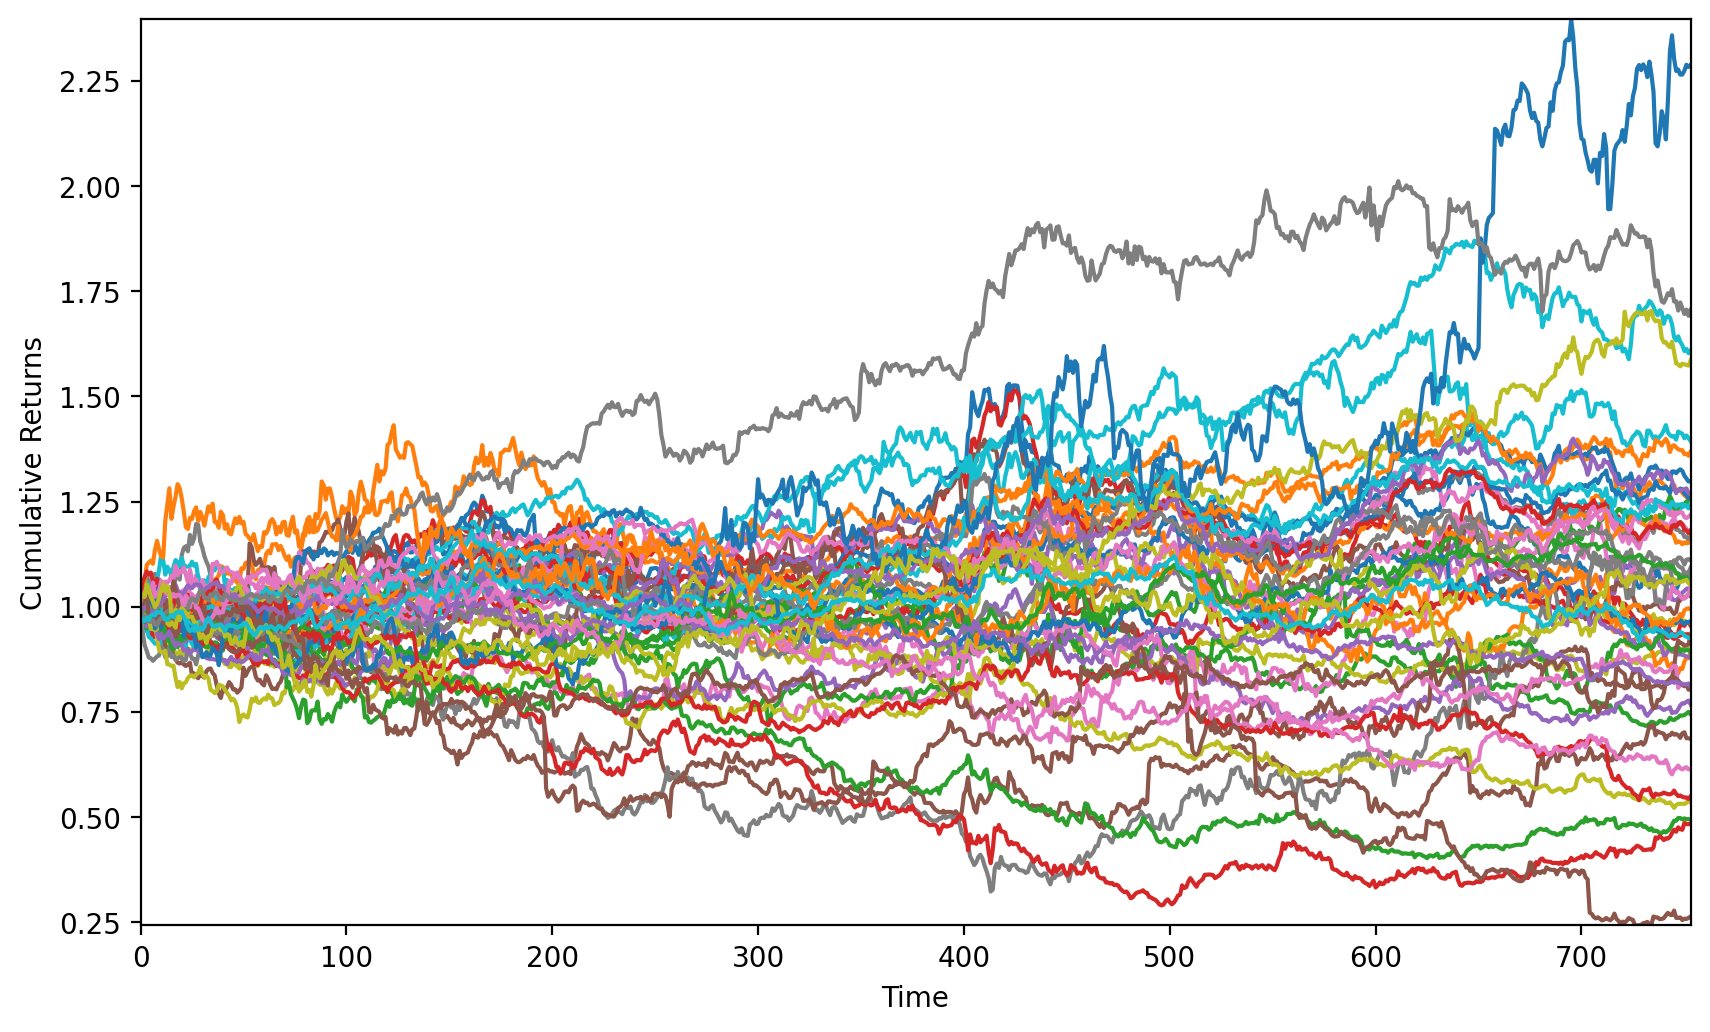
\includegraphics[width=0.8\textwidth]{images/cumulative_returns_qrt_timeseries_data.png}
%     \caption{Cumulative Returns for Daily Returns Time Series}
%     \label{fig:cumulative_returns}
% \end{figure}
% \begin{figure}[htbp]
%   \centering
%   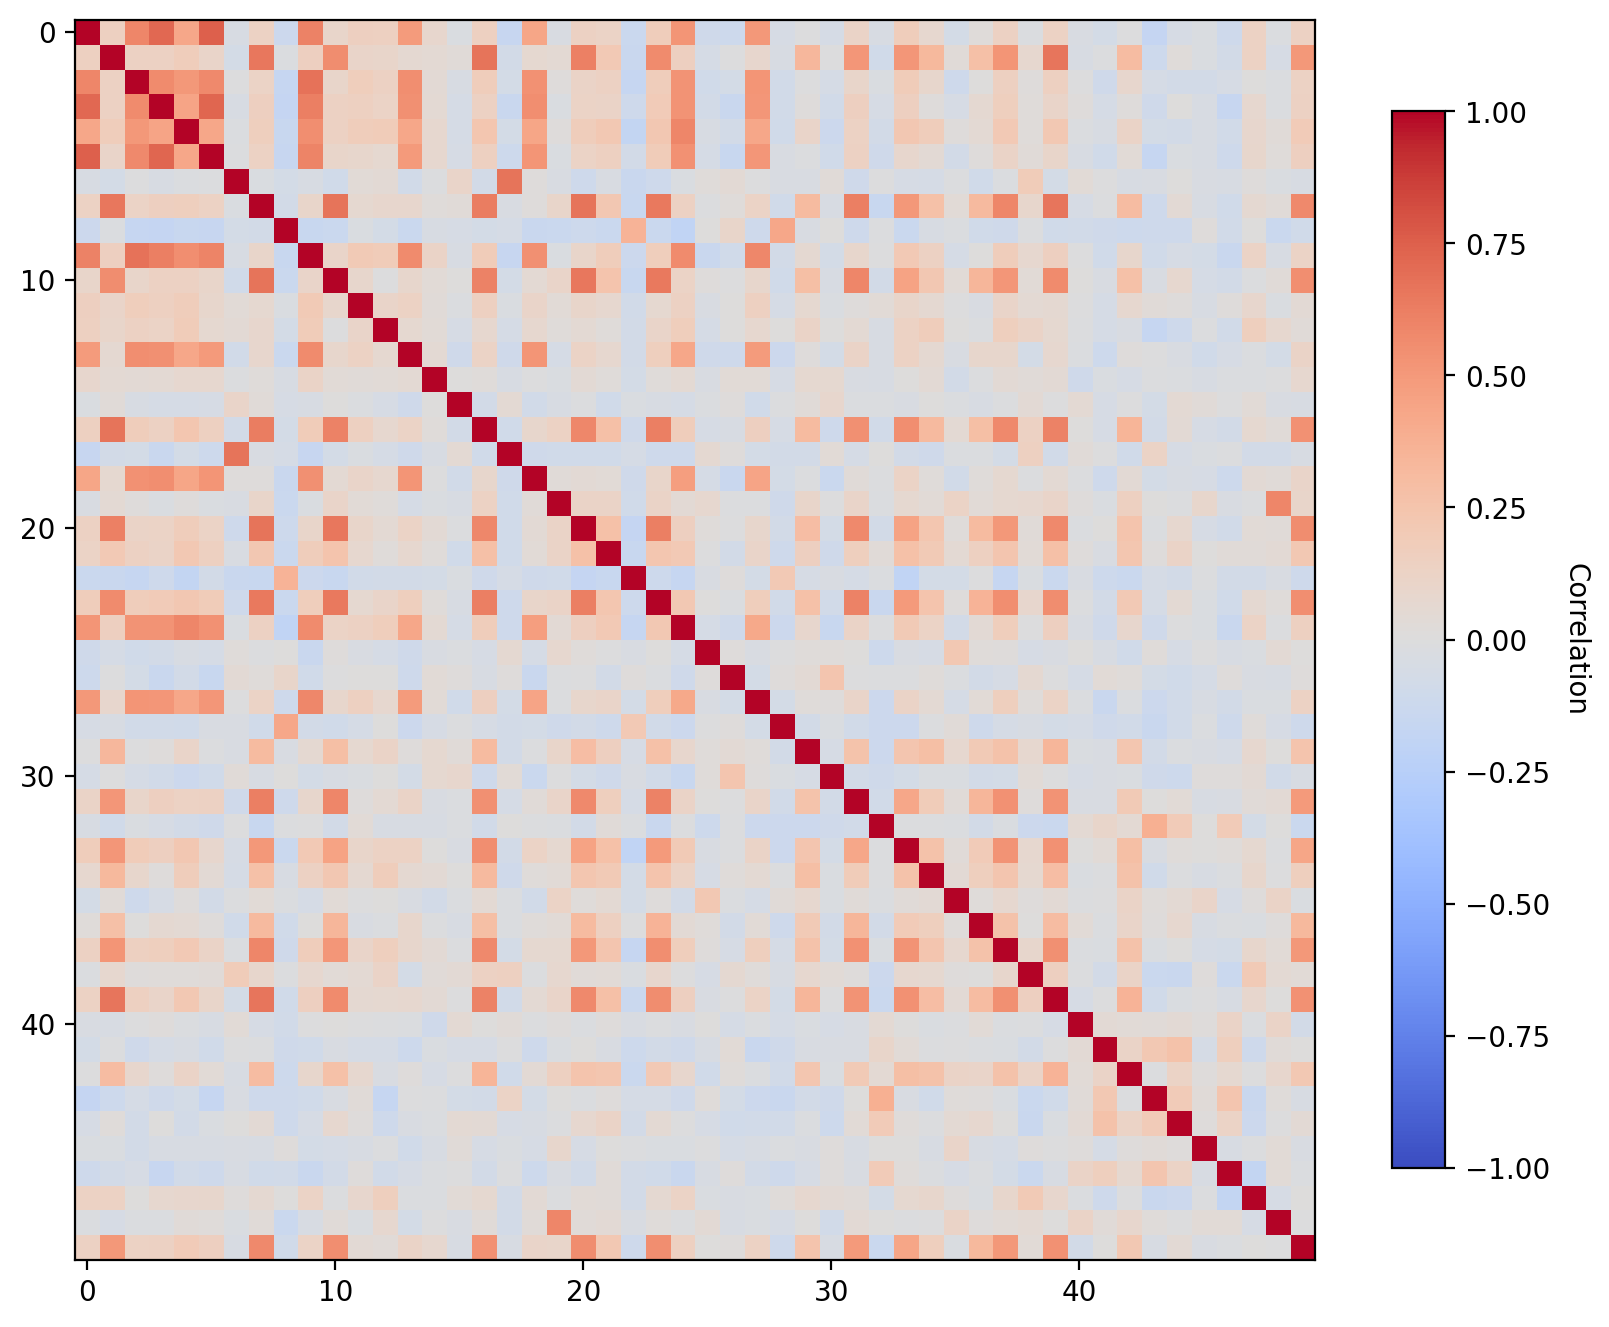
\includegraphics[width=0.9\textwidth]{images/correlation_matrix_50by50_timeseries_qtr_data.png}
%   \caption{Correlation Matrix for returns of 50 time series}
%   \label{fig:corr_matrix_ts_qrt_data}
% \end{figure}

\begin{figure}[H]
    \centering
    \begin{minipage}[t]{0.5789\textwidth}
        \centering
        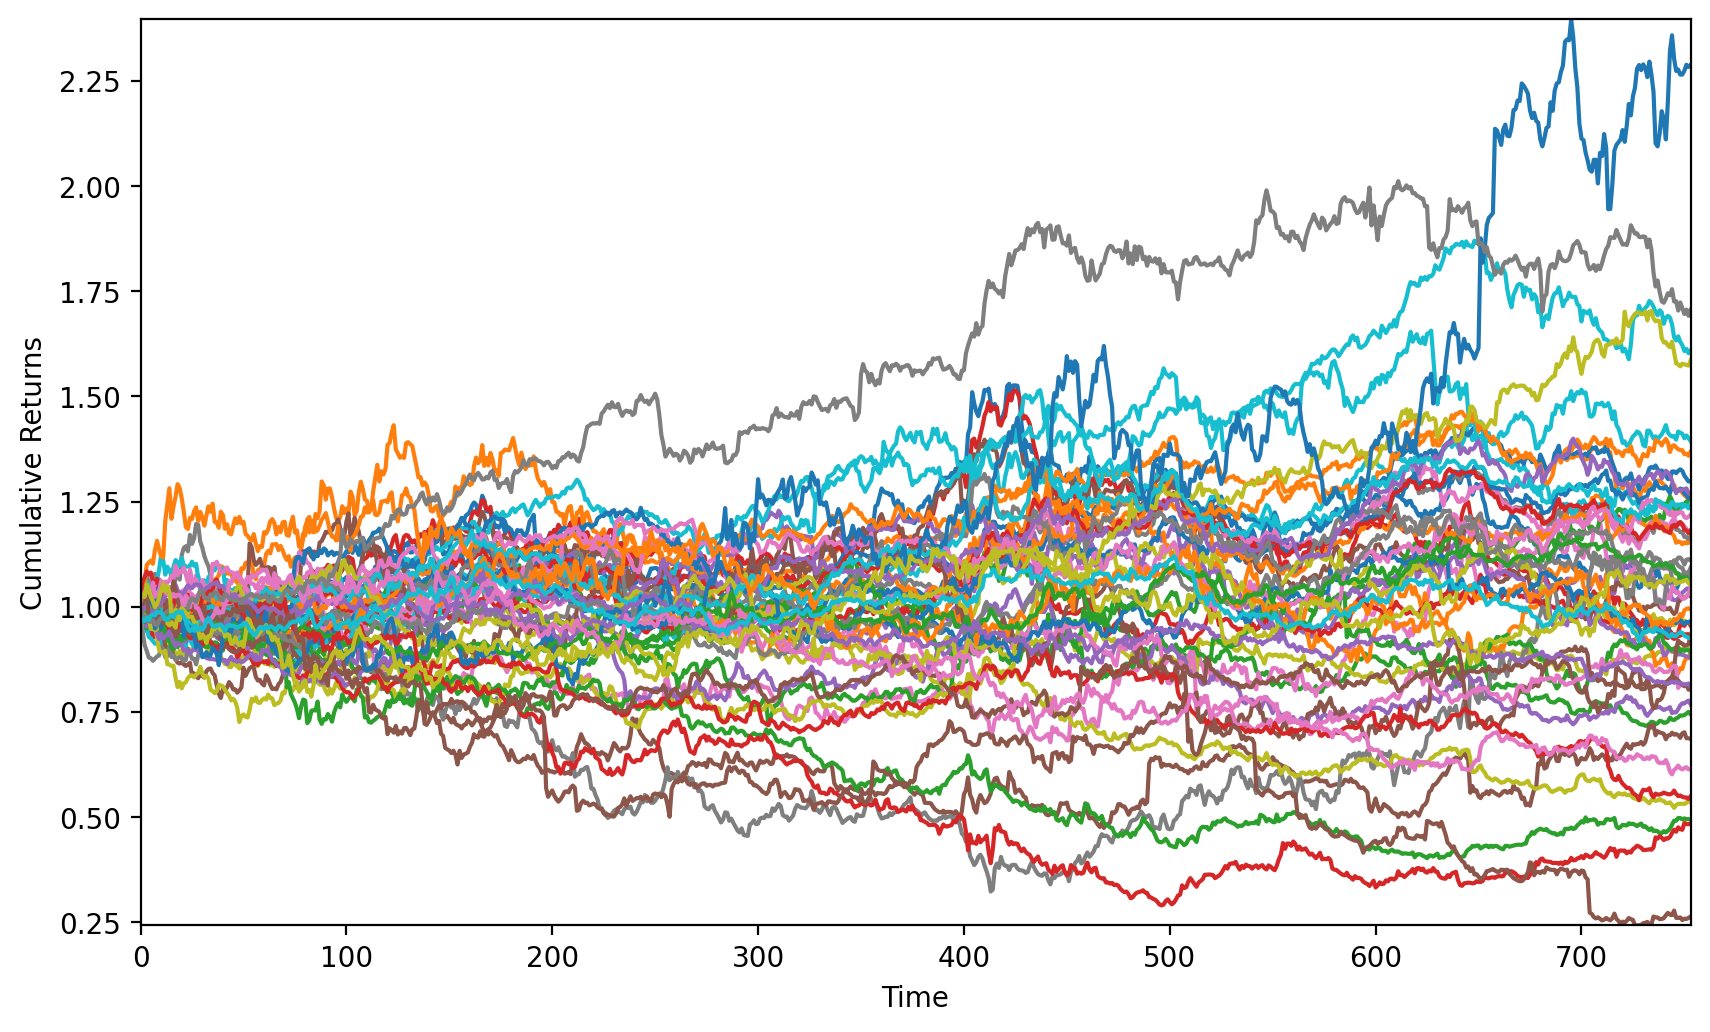
\includegraphics[width=\textwidth]{images/cumulative_returns_qrt_timeseries_data.png}
        \captionsetup{font=tiny}
        \caption{Cumulative Returns for Daily Returns Time Series}
        \label{fig:cumulative_returns}
    \end{minipage}%
    \begin{minipage}[t]{0.4211\textwidth}
        \centering
        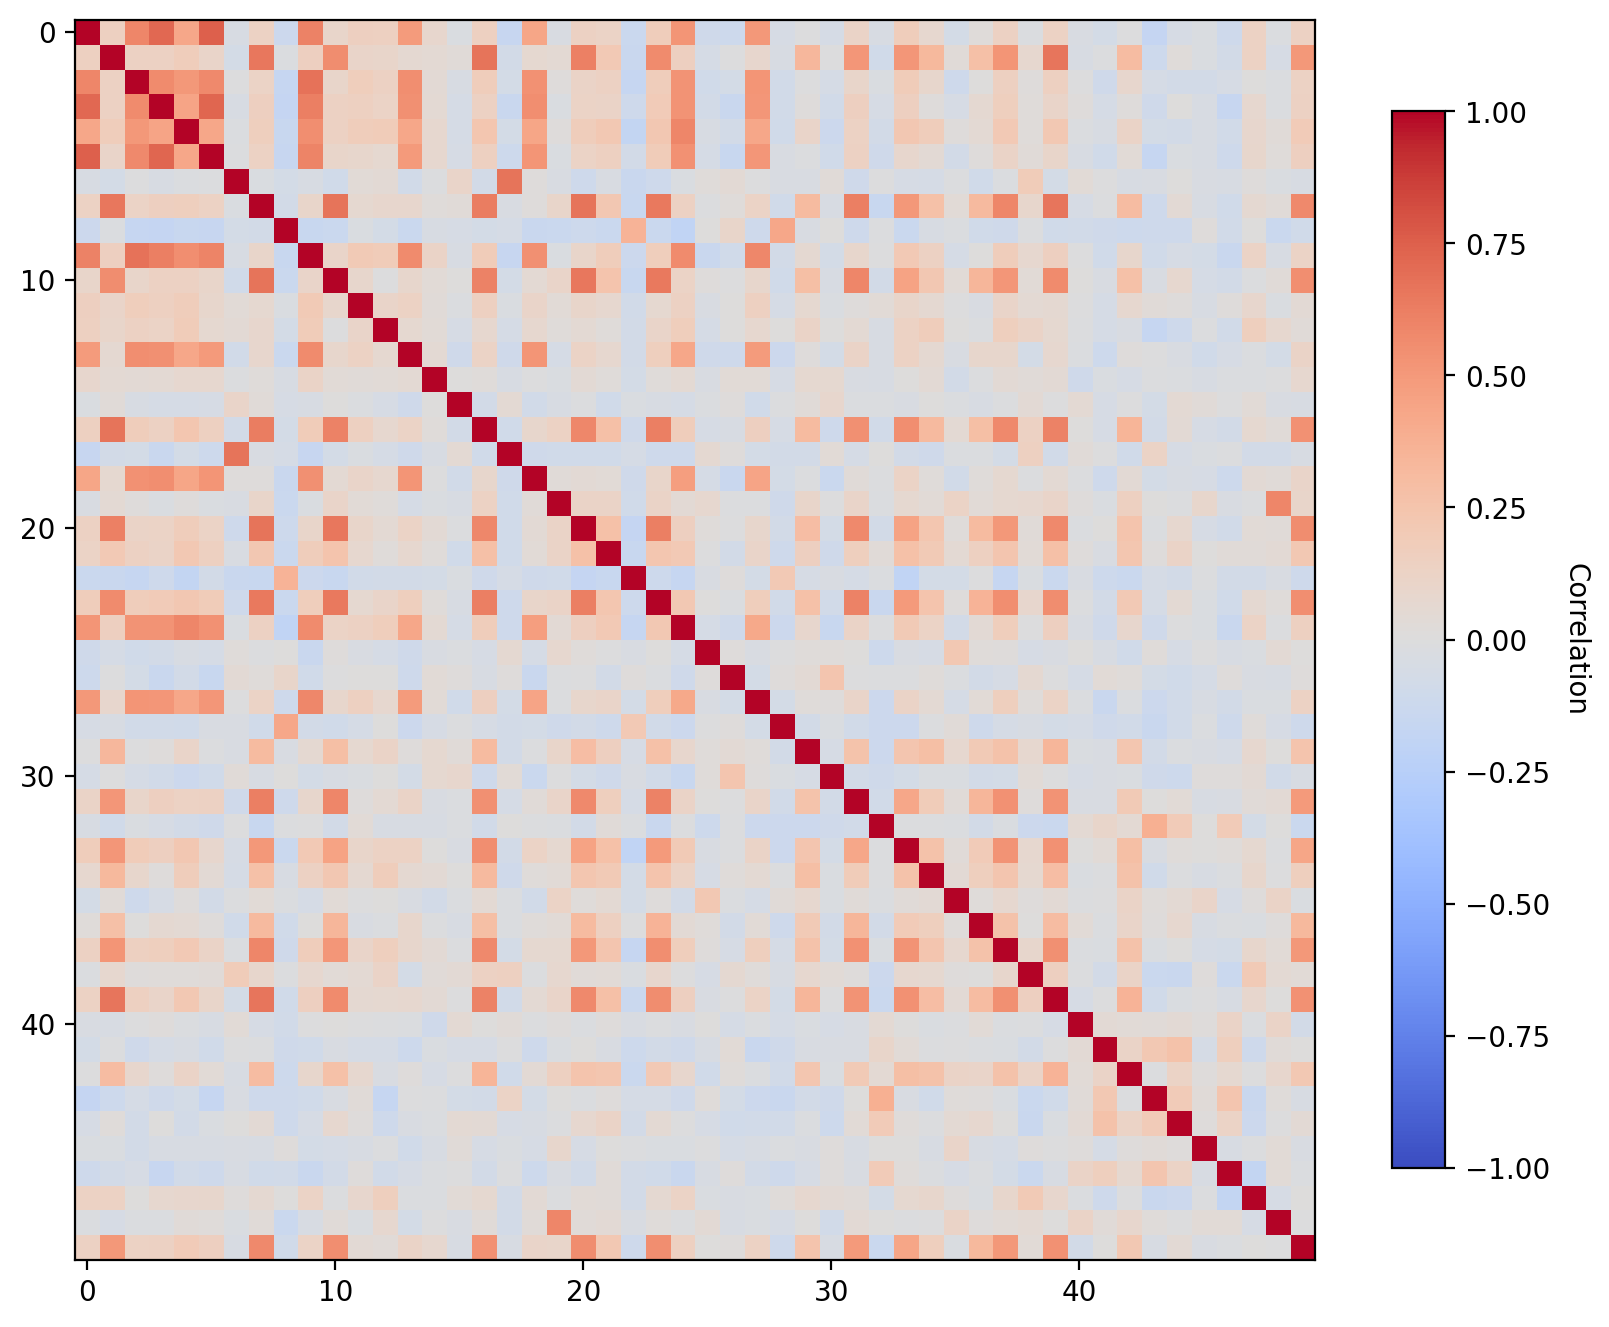
\includegraphics[width=\textwidth]{images/correlation_matrix_50by50_timeseries_qtr_data.png}
        \captionsetup{font=tiny}
        \caption{Correlation Matrix of Daily Returns}
        \label{fig:corr_matrix_ts_qrt_data}
    \end{minipage}
\end{figure}
\begin{figure}[H]
  \centering
  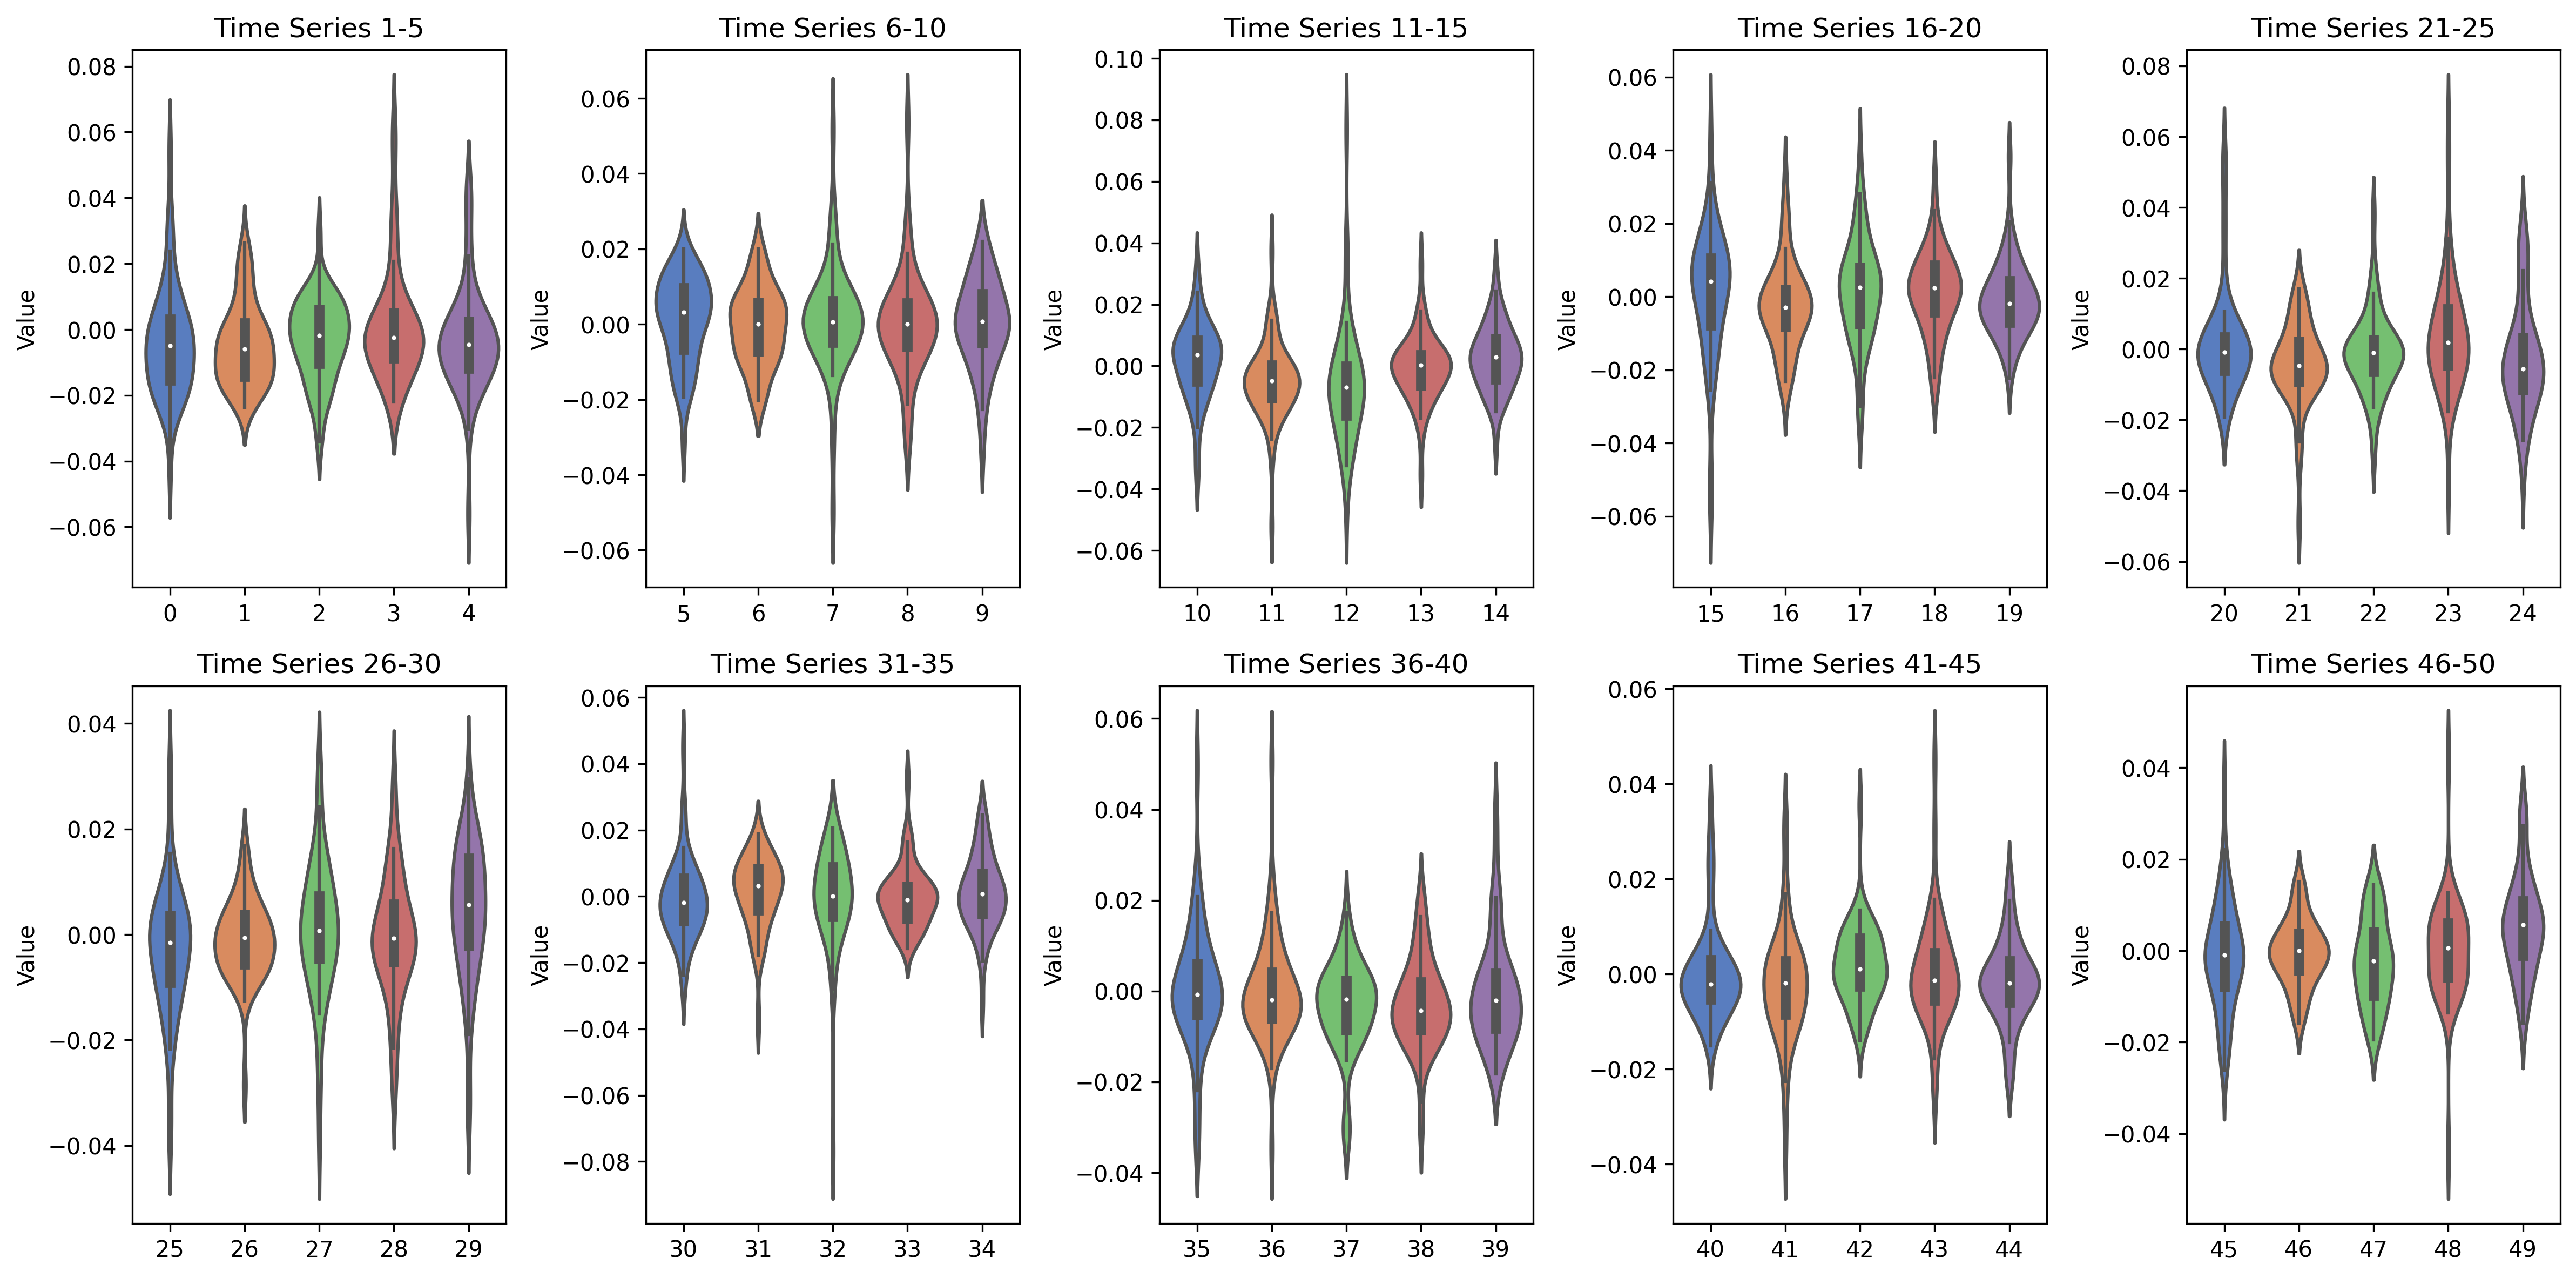
\includegraphics[width=\textwidth]{images/violin_plots_50_timeseries.png}
  \caption{Violin Plots for 50 Time Series}
  \label{fig:violin_plots}
\end{figure}

\level{3}{Preprocessing}

For statistical significance of results we will use multiple samples from the set of 50 timeseries for $n = 5,8,13,21,34,50$ being the sample sizes and $m=10,7,4,3,1$ being the number of such samples for each $n$.
































% \newpage
% %%% ADVERSARIAL NETWORK
% \level{2}{Problem: Defense Against Adversarial Attack} \label{results_problem_2} 
% \hspace{6mm} A dataset of $n$ images ${(X_1, y_1), (X_2, y_2), ..., (X_n, y_n)}$, where $X_i$ represents an image and $y_i$ represents its corresponding label, the task is to develop a function $N(X_i; \theta)$ that takes an image $X_i$ as input and predicts its label $y_i$ using a set of model parameters $\theta$.
% \newline Formally, the task is to find the optimal set of parameters $\theta^*$ that minimizes the following loss function:
% \begin{equation} \label{problem_daaamd_opt_thita_expression}
%     \theta^* = \arg\min_\theta \frac{1}{n}\sum_{i=1}^n L(N(X_i; \theta), y_i)
% \end{equation}
% \newline where $L$ is a loss function that measures the difference between the predicted label and the true label.

% An adversarial attack is a perturbation $\delta$ added to the original input image $X_i$ to produce a new image $X_i' = X_i + \delta$ that is designed to cause misclassification of the model. The goal of the attacker is to find the perturbation $\delta$ that maximizes the difference between the predicted label and the true label.
% \newline Formally, the task is to find the optimal perturbation $\delta^*$ that maximizes the following objective function:
% \begin{equation} \label{problem_daaamd_adv_delta_expression}
%     \delta^* = \arg\max_\delta L(N(X_i + \delta; \theta), y_i)
% \end{equation}
% \newline where $L$ is a loss function that measures the difference between the predicted label and the true label.

% \level{3}{Data}
% The MNIST dataset consists of 60,000 grayscale images of handwritten digits (0-9) with a resolution of 28x28 pixels. There is an additional test set of 10,000 images. Each image is labeled with its corresponding digit. The pixel intensity values of the images in the MNIST dataset range over integer values from 0 to 255. 
% \newline 
% The MNIST dataset is a widely used benchmark dataset in the field of machine learning, and many different models have been developed to classify the digits in this dataset. However, it has been shown that these models are vulnerable to adversarial attacks, which can cause them to misclassify images with high confidence.

% \begin{figure}[H]
%   \centering
%   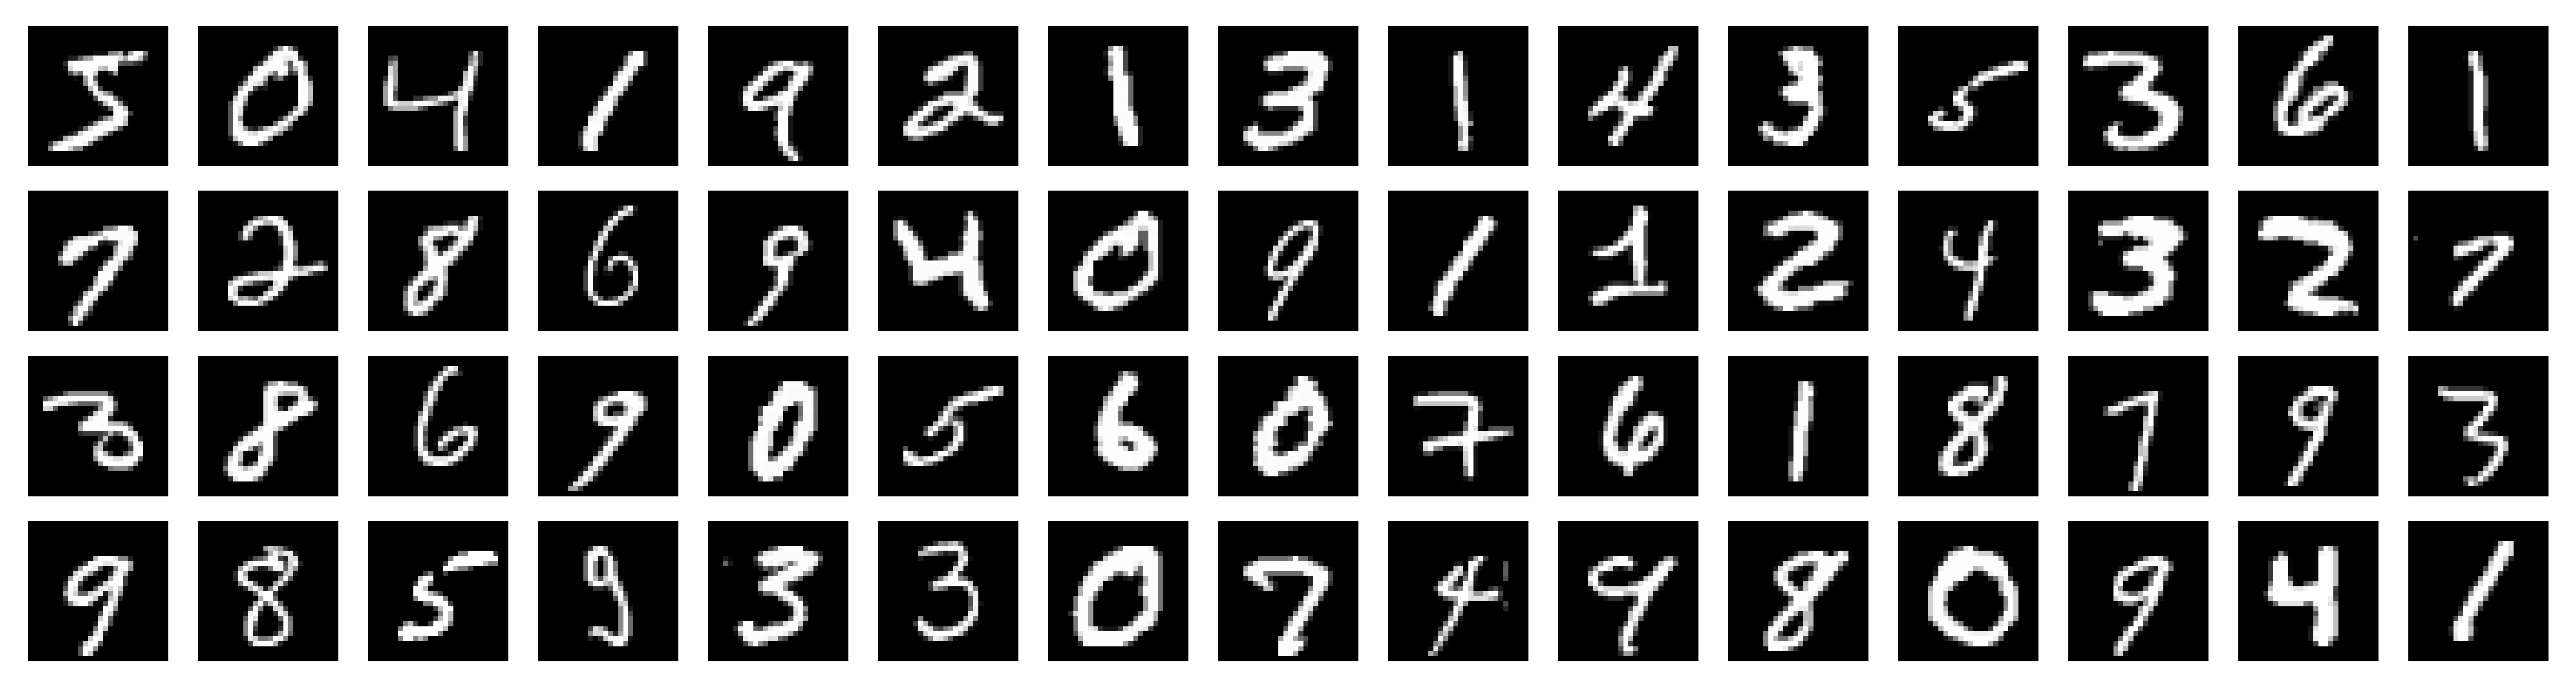
\includegraphics[width=0.9\textwidth]{images/mnist_60_images_4x15_grid.png}
%   \caption{Images from the MNIST training set.}
%   \label{fig:mnist_images}
% \end{figure}

% \level{4}{Preprocessing }

% \level{3}{Approaches}
% \level{4}{Linear Classifier}
% \level{4}{Linear Classifier with $L_2$ Norm}
% \level{4}{Linear Classifier with $\kappa_2$ Minimization}


